%DIF 1-12c1
%DIF LATEXDIFF DIFFERENCE FILE
%DIF DEL uo2_tdeA.tex   Mon Feb 11 09:53:26 2019
%DIF ADD uo2_tde.tex    Mon Feb 11 09:21:36 2019
%DIF < \documentclass[8pt]{article}   	% use "amsart" instead of "article" for AMSLaTeX format
%DIF < \usepackage{geometry}                		% See geometry.pdf to learn the layout options. There are lots.
%DIF < \geometry{letterpaper}                   		% ... or a4paper or a5paper or ...
%DIF < %\geometry{landscape}                		% Activate for rotated page geometry
%DIF < %\usepackage[parfill]{parskip}    		% Activate to begin paragraphs with an empty line rather than an indent
%DIF < \usepackage{graphicx}				% Use pdf, png, jpg, or eps§ with pdflatex; use eps in DVI mode
%DIF < 								% TeX will automatically convert eps --> pdf in pdflatex
%DIF < \usepackage{amssymb}
%DIF < \usepackage{cite}
%DIF < \usepackage{subfigure}
%DIF < \usepackage{float}
%DIF < \usepackage{placeins}
%DIF -------
\documentclass[review]{elsarticle} %DIF > 
%DIF -------
\usepackage{hyperref}
%DIF 14a3-5
\usepackage[margin=1in]{geometry} %DIF > 
\usepackage{graphicx} %DIF > 
\usepackage{amsmath} %DIF > 
%DIF -------
\usepackage{placeins}
\usepackage{comment}
%DIF 16-18c8
%DIF < \usepackage{gensymb}
%DIF < \usepackage{lineno}
%DIF < \usepackage{authblk}
%DIF -------
\usepackage{fancyref} %DIF > 
%DIF -------
\usepackage{color}
%DIF 20a10
\usepackage{multirow} %DIF > 
%DIF -------

%DIF 21c12
%DIF < %\date{}							% Activate to display a given date or no date
%DIF -------
\def\bibsection{\section*{References}} %DIF > 
%DIF -------

%DIF < \title{Calculation of Threshold Displacement Energies in $UO_2$}
%DIF -------
\journal{Journal of Nuclear Materials} %DIF > 
%DIF < \author[1]{Benjamin Dacus}
\bibliographystyle{elsarticle-num} %DIF > 
%DIF < \author[2]{Benjamin Beeler}
%DIF < \author[2]{Daniel Schwen}
%DIF < 
%DIF < \affil[1]{North Carolina State University, Raleigh, NC 27695}
%DIF < \affil[2]{Idaho National Laboratory, Idaho Falls, ID 83415}
%DIF PREAMBLE EXTENSION ADDED BY LATEXDIFF
%DIF CTRADITIONAL PREAMBLE %DIF PREAMBLE
\RequirePackage{color}\definecolor{RED}{rgb}{1,0,0}\definecolor{BLUE}{rgb}{0,0,1} %DIF PREAMBLE
\RequirePackage[stable]{footmisc} %DIF PREAMBLE
\DeclareOldFontCommand{\sf}{\normalfont\sffamily}{\mathsf} %DIF PREAMBLE
\providecommand{\DIFaddtex}[1]{{\protect\color{blue} \sf #1}} %DIF PREAMBLE
\providecommand{\DIFdeltex}[1]{{\protect\color{red} [..\footnote{removed: #1} ]}} %DIF PREAMBLE
%DIF SAFE PREAMBLE %DIF PREAMBLE
\providecommand{\DIFaddbegin}{} %DIF PREAMBLE
\providecommand{\DIFaddend}{} %DIF PREAMBLE
\providecommand{\DIFdelbegin}{} %DIF PREAMBLE
\providecommand{\DIFdelend}{} %DIF PREAMBLE
%DIF FLOATSAFE PREAMBLE %DIF PREAMBLE
\providecommand{\DIFaddFL}[1]{\DIFadd{#1}} %DIF PREAMBLE
\providecommand{\DIFdelFL}[1]{\DIFdel{#1}} %DIF PREAMBLE
\providecommand{\DIFaddbeginFL}{} %DIF PREAMBLE
\providecommand{\DIFaddendFL}{} %DIF PREAMBLE
\providecommand{\DIFdelbeginFL}{} %DIF PREAMBLE
\providecommand{\DIFdelendFL}{} %DIF PREAMBLE
%DIF HYPERREF PREAMBLE %DIF PREAMBLE
\providecommand{\DIFadd}[1]{\texorpdfstring{\DIFaddtex{#1}}{#1}} %DIF PREAMBLE
\providecommand{\DIFdel}[1]{\texorpdfstring{\DIFdeltex{#1}}{}} %DIF PREAMBLE
\newcommand{\DIFscaledelfig}{0.5}
%DIF HIGHLIGHTGRAPHICS PREAMBLE %DIF PREAMBLE
\RequirePackage{settobox} %DIF PREAMBLE
\RequirePackage{letltxmacro} %DIF PREAMBLE
\newsavebox{\DIFdelgraphicsbox} %DIF PREAMBLE
\newlength{\DIFdelgraphicswidth} %DIF PREAMBLE
\newlength{\DIFdelgraphicsheight} %DIF PREAMBLE
% store original definition of \includegraphics %DIF PREAMBLE
\LetLtxMacro{\DIFOincludegraphics}{\includegraphics} %DIF PREAMBLE
\newcommand{\DIFaddincludegraphics}[2][]{{\color{blue}\fbox{\DIFOincludegraphics[#1]{#2}}}} %DIF PREAMBLE
\newcommand{\DIFdelincludegraphics}[2][]{% %DIF PREAMBLE
\sbox{\DIFdelgraphicsbox}{\DIFOincludegraphics[#1]{#2}}% %DIF PREAMBLE
\settoboxwidth{\DIFdelgraphicswidth}{\DIFdelgraphicsbox} %DIF PREAMBLE
\settoboxtotalheight{\DIFdelgraphicsheight}{\DIFdelgraphicsbox} %DIF PREAMBLE
\scalebox{\DIFscaledelfig}{% %DIF PREAMBLE
\parbox[b]{\DIFdelgraphicswidth}{\usebox{\DIFdelgraphicsbox}\\[-\baselineskip] \rule{\DIFdelgraphicswidth}{0em}}\llap{\resizebox{\DIFdelgraphicswidth}{\DIFdelgraphicsheight}{% %DIF PREAMBLE
\setlength{\unitlength}{\DIFdelgraphicswidth}% %DIF PREAMBLE
\begin{picture}(1,1)% %DIF PREAMBLE
\thicklines\linethickness{2pt} %DIF PREAMBLE
{\color[rgb]{1,0,0}\put(0,0){\framebox(1,1){}}}% %DIF PREAMBLE
{\color[rgb]{1,0,0}\put(0,0){\line( 1,1){1}}}% %DIF PREAMBLE
{\color[rgb]{1,0,0}\put(0,1){\line(1,-1){1}}}% %DIF PREAMBLE
\end{picture}% %DIF PREAMBLE
}\hspace*{3pt}}} %DIF PREAMBLE
} %DIF PREAMBLE
\LetLtxMacro{\DIFOaddbegin}{\DIFaddbegin} %DIF PREAMBLE
\LetLtxMacro{\DIFOaddend}{\DIFaddend} %DIF PREAMBLE
\LetLtxMacro{\DIFOdelbegin}{\DIFdelbegin} %DIF PREAMBLE
\LetLtxMacro{\DIFOdelend}{\DIFdelend} %DIF PREAMBLE
\DeclareRobustCommand{\DIFaddbegin}{\DIFOaddbegin \let\includegraphics\DIFaddincludegraphics} %DIF PREAMBLE
\DeclareRobustCommand{\DIFaddend}{\DIFOaddend \let\includegraphics\DIFOincludegraphics} %DIF PREAMBLE
\DeclareRobustCommand{\DIFdelbegin}{\DIFOdelbegin \let\includegraphics\DIFdelincludegraphics} %DIF PREAMBLE
\DeclareRobustCommand{\DIFdelend}{\DIFOaddend \let\includegraphics\DIFOincludegraphics} %DIF PREAMBLE
\LetLtxMacro{\DIFOaddbeginFL}{\DIFaddbeginFL} %DIF PREAMBLE
\LetLtxMacro{\DIFOaddendFL}{\DIFaddendFL} %DIF PREAMBLE
\LetLtxMacro{\DIFOdelbeginFL}{\DIFdelbeginFL} %DIF PREAMBLE
\LetLtxMacro{\DIFOdelendFL}{\DIFdelendFL} %DIF PREAMBLE
\DeclareRobustCommand{\DIFaddbeginFL}{\DIFOaddbeginFL \let\includegraphics\DIFaddincludegraphics} %DIF PREAMBLE
\DeclareRobustCommand{\DIFaddendFL}{\DIFOaddendFL \let\includegraphics\DIFOincludegraphics} %DIF PREAMBLE
\DeclareRobustCommand{\DIFdelbeginFL}{\DIFOdelbeginFL \let\includegraphics\DIFdelincludegraphics} %DIF PREAMBLE
\DeclareRobustCommand{\DIFdelendFL}{\DIFOaddendFL \let\includegraphics\DIFOincludegraphics} %DIF PREAMBLE
%DIF END PREAMBLE EXTENSION ADDED BY LATEXDIFF

\begin{document}
\DIFaddbegin \begin{frontmatter}
\DIFaddend 


\DIFdelbegin %DIFDELCMD < \begin{comment}%DIFDELCMD < 
%DIFDELCMD < \author[ncst]{Benjamin Dacus}
%DIFDELCMD < \author[inl]{Benjamin Beeler}
%DIFDELCMD < \author[inl]{Daniel Schwen}
%DIFDELCMD < \address[inl]{Idaho National Laboratory, Idaho Falls, ID 83415}
%DIFDELCMD < \address[ncst]{North Carolina State University, Raleigh, NC 27695}
%DIFDELCMD < \end{comment}
%DIFDELCMD < %%%
\DIFdelend \DIFaddbegin \title{\DIFadd{Calculation of Threshold Displacement Energies in UO$_2$}}
\DIFaddend 



\DIFdelbegin %DIFDELCMD < \begin{@twocolumnfalse}
%DIFDELCMD < \maketitle
%DIFDELCMD <     %%%
\DIFdelend \DIFaddbegin \author[ncst]{\DIFadd{Benjamin Dacus}}
\author[inl]{\DIFadd{Benjamin Beeler}\corref{qwe}}
\cortext[qwe]{Corresponding author}
\author[inl]{\DIFadd{Daniel Schwen}}
\address[inl]{Idaho National Laboratory, Idaho Falls, ID 83415}
\address[ncst]{North Carolina State University, Raleigh, NC 27695}





  \DIFaddend \begin{abstract}
   Despite the extensive utilization of uranium dioxide (\DIFdelbegin \DIFdel{$UO_2$}\DIFdelend \DIFaddbegin \DIFadd{UO$_2$}\DIFaddend ) as a \DIFdelbegin \DIFdel{driver }\DIFdelend fuel in commercial nuclear reactors, there is only minimal information regarding the fundamental nature of radiation damage at high temperatures, such as those experienced by the fuel under operation. In this work, molecular dynamics simulations have been performed to determine the threshold displacement energy (\DIFdelbegin \DIFdel{$E_d$}\DIFdelend \DIFaddbegin \DIFadd{E$_d$}\DIFaddend ) for oxygen and uranium in \DIFdelbegin \DIFdel{$UO_2$ }\DIFdelend \DIFaddbegin \DIFadd{UO$_2$ }\DIFaddend at 1500 K. Three definitions of displacement energy were employed to fully study the nature of low energy radiation damage: 1) the probability of \DIFdelbegin \DIFdel{forming a stable Frenkel defect, 2) the probability of }\DIFdelend having the primary knock-on atom (PKA) leave its original lattice site, \DIFdelbegin \DIFdel{and 3) the number of permanently displaced atoms due to the PKA}\DIFdelend \DIFaddbegin \DIFadd{2) the probability that the PKA will permanently displace atoms from their original lattice site, and 3) the probability of forming a stable Frenkel pair}\DIFaddend . Additionally, \DIFdelbegin \DIFdel{three }\DIFdelend \DIFaddbegin \DIFadd{four }\DIFaddend unique interatomic potentials were utilized to \DIFdelbegin \DIFdel{determine }\DIFdelend \DIFaddbegin \DIFadd{investigate }\DIFaddend uncertainties associated with potential choice in high temperature radiation damage studies in \DIFdelbegin \DIFdel{$UO_2$}\DIFdelend \DIFaddbegin \DIFadd{UO$_2$}\DIFaddend . This work provides critical insight into the high temperature behavior of radiation damage in \DIFdelbegin \DIFdel{$UO_2$}\DIFdelend \DIFaddbegin \DIFadd{UO$_2$}\DIFaddend , as well as the variation in behavior between oxygen and uranium PKAs.
  \end{abstract}
\DIFdelbegin %DIFDELCMD < \end{@twocolumnfalse}
%DIFDELCMD < %%%
\DIFdelend 


\DIFaddbegin \end{frontmatter}

\DIFaddend \clearpage
\newpage

\section{Introduction}

\hspace{5mm}
Due to its usage as a nuclear fuel, uranium dioxide (\DIFdelbegin \DIFdel{$UO_2$}\DIFdelend \DIFaddbegin \DIFadd{UO$_2$}\DIFaddend ) has been thoroughly studied both theoretically and experimentally over the the last half-century. Utilization of this data can provide correlations for a range of thermo-mechanical behaviors, and such correlations can serve as inputs to continuum-level fuel performance modeling. Such fuel performance models \cite{williamson_et_al_2012, falcon04, bentejac2004, thouvenin2007, sercombe2009} have shown impressive accuracy in their ability to describe fuel behavior. However, fuel performance models that rely on empirical correlations are inherently limited in their applicability to the scope of the data used to construct those empirical models. In order to predict fuel behavior in scenarios outside of the existing experimental data regimes, the underlying physics of the material systems needs to be included into the fuel performance models. This can be done by informing continuum level simulations with mesoscale and atomistic data taking into account the microstructural evolution of the material.

In addition to very high neutron flux and fluence during operation, nuclear fuels are exposed to high energy fission fragments and alpha particles released during radioactive decay of fission products. The ability to quantify the damage resulting from this radiation is a critical step in describing and understanding microstructural evolution of nuclear fuel. The threshold displacement energy (\DIFdelbegin \DIFdel{$E_d$}\DIFdelend \DIFaddbegin \DIFadd{E$_d$}\DIFaddend ) is a critical measure of a material's response to radiation damage. The amount of damage that a material system experiences under irradiation is typically described in displacements per atom (dpa). Models such as the Norgett-Robinson-Torrens (NRT) \cite{nrt} utilize a threshold displacement energy to calculate a given \textit{dpa} based on the material and irradiation condition. \DIFaddbegin \DIFadd{For a multicomponent system an effective displacement energy needs to be utilized in the NRT model \cite{crocombette2016}, while the more rigorous approach by Parkin and Coulter \cite{PC1980} requires a displacement energy for each component. }\DIFaddend It is thus critical to possess an accurate description of \DIFdelbegin \DIFdel{$E_d$ }\DIFdelend \DIFaddbegin \DIFadd{E$_d$ }\DIFaddend in order to accurately assess the number of \textit{dpa} the material system of interest experiences.

There have been several investigations over the past three decades studying \DIFdelbegin \DIFdel{$E_d$ in $UO_2$}\DIFdelend \DIFaddbegin \DIFadd{E$_d$ in UO$_2$}\DIFaddend . Using transmission electron microscopy on room temperature \DIFdelbegin \DIFdel{$UO_2$ }\DIFdelend \DIFaddbegin \DIFadd{UO$_2$ }\DIFaddend samples, Soullard \cite{soullard1977,soullard1985} determined that the threshold displacement energies in \DIFdelbegin \DIFdel{$UO_2$ }\DIFdelend \DIFaddbegin \DIFadd{UO$_2$ }\DIFaddend are 20 eV for oxygen primary knock-on atoms (PKAs) and 40 eV for uranium PKAs. However, this work makes usage of a variety of assumptions, including the validity of the Kinchin-Pease model, extrapolation of dislocation loops to the number of point defects and that the oxygen \DIFdelbegin \DIFdel{$E_d$ }\DIFdelend \DIFaddbegin \DIFadd{E$_d$ }\DIFaddend is half that of the uranium \DIFdelbegin \DIFdel{$E_d$}\DIFdelend \DIFaddbegin \DIFadd{E$_d$}\DIFaddend . Additionally, Soullard only reports that the uranium \DIFdelbegin \DIFdel{$E_d$ }\DIFdelend \DIFaddbegin \DIFadd{E$_d$ }\DIFaddend is ``on the order of 40 eV." These are the only known experimental studies on \DIFdelbegin \DIFdel{$E_d$ in $UO_2$. }\DIFdelend \DIFaddbegin \DIFadd{E$_d$ in UO$_2$. Therefore there are no experimental studies on the value of E$_d$ for O PKAs in UO$_2$.
}\DIFaddend 

Computationally, Meis and Chartier \cite{meis2005} used the sudden approximation method within the Mott-Littleton approach \cite{Litt} in order to determine \DIFdelbegin \DIFdel{$E_d$}\DIFdelend \DIFaddbegin \DIFadd{E$_d$}\DIFaddend . They determined that the value of \DIFdelbegin \DIFdel{$E_d$ }\DIFdelend \DIFaddbegin \DIFadd{E$_d$ }\DIFaddend for oxygen PKAs (\DIFdelbegin \DIFdel{$E_d [O]$}\DIFdelend \DIFaddbegin \DIFadd{E$_d$}[\DIFadd{O}]\DIFaddend ) is approximately 20 eV, and \DIFdelbegin \DIFdel{$E_d$ }\DIFdelend \DIFaddbegin \DIFadd{E$_d$ }\DIFaddend for uranium PKAs (\DIFdelbegin \DIFdel{$E_d [U]$}\DIFdelend \DIFaddbegin \DIFadd{E$_d$}[\DIFadd{U}]\DIFaddend ) is approximately 50 eV. Molecular dynamics simulations have also been employed to investigate radiation damage in \DIFdelbegin \DIFdel{$UO_2$}\DIFdelend \DIFaddbegin \DIFadd{UO$_2$}\DIFaddend , although not specifically \DIFdelbegin \DIFdel{$E_d$}\DIFdelend \DIFaddbegin \DIFadd{E$_d$}\DIFaddend . Van Brutzel \cite{vanbrutzel2003,vanbrutzel2006} and Martin et al \cite{martin2011} performed radiation damage simulations for PKA energies of up to 100 keV at 300 K and compared their results to the NRT correlation for an \DIFdelbegin \DIFdel{$E_d$ }\DIFdelend \DIFaddbegin \DIFadd{E$_d$ }\DIFaddend value of 30 eV (averaged over the experimental \DIFdelbegin \DIFdel{results }\DIFdelend \DIFaddbegin \DIFadd{approximations }\DIFaddend of 20 eV for O and 40 eV for U). It is interesting to note that Van Brutzel determined that the linear NRT \DIFdelbegin \DIFdel{corelation }\DIFdelend \DIFaddbegin \DIFadd{correlation }\DIFaddend was not valid at higher energies due to the recombination of defects and that the number of defects instead follows a power law, but Martin showed that a linear relationship is retained at high PKA energies. Devanathan \cite{devanathan2009} conducted 1 keV cascade simulations at 300 K utilizing five different interatomic potentials and extrapolated the displacement energy from the modified Kinchin-Pease equation \cite{kinchinpease}. Martin \cite{martin2015, martin2014} studied the effect of temperature on displacement cascades using the Morelon \cite{morelon2003} potential. The authors are unaware of any attempts to investigate the nature of \DIFdelbegin \DIFdel{$E_d$ in $UO_2$ }\DIFdelend \DIFaddbegin \DIFadd{E$_d$ in UO$_2$ }\DIFaddend at high temperatures. We note that all these studies employ the basic monoatomic NRT model which is not rigorously applicable to the diatomic UO$_2$, which has two constituents that have very different $Z$ values and thus very different charged particle scattering cross sections.

Although \DIFdelbegin \DIFdel{$E_d$ }\DIFdelend \DIFaddbegin \DIFadd{E$_d$ }\DIFaddend has been extensively studied computationally, there still exist some discrepancies with regard to how individual researchers define \DIFdelbegin \DIFdel{$E_d$}\DIFdelend \DIFaddbegin \DIFadd{E$_d$}\DIFaddend . Meis and Chartier \cite{meis2005} define \DIFdelbegin \DIFdel{$E_d$ }\DIFdelend \DIFaddbegin \DIFadd{E$_d$ }\DIFaddend as the "minimum energy transferred to a lattice atom along a given crystallographic direction yielding the creation of a stable Frenkel defect". However, other authors such as Devanathan \cite{devanathan1998} define the threshold displacement energy as "the minimum energy needed to displace an atom from its lattice site." This definition from Devanathan is yet unclear with respect to how displacement is defined. For instance, the energy required to remove an atom from a lattice site \textit{permanently} is higher than the energy required to remove an atom from is lattice site and have it eventually return. \DIFdelbegin \DIFdel{A }\DIFdelend \DIFaddbegin \DIFadd{Perhaps a }\DIFaddend more precise definition is described by Motta \cite{Motta} where \DIFdelbegin \DIFdel{$E_d$ }\DIFdelend \DIFaddbegin \DIFadd{E$_d$ }\DIFaddend is "the minimum energy required to sufficiently move the atoms so that they do not return to their initial sites". It should be noted that this definition from Motta does not necessarily indicate the generation of a stable Frenkel pair. It is worth investigating all three definitions (generation of a Frenkel pair, displacement off initial lattice site, permanent displacement off initial lattice site) of the threshold displacement energy separately in order to ascertain the differences in the \DIFdelbegin \DIFdel{hopes }\DIFdelend \DIFaddbegin \DIFadd{hope }\DIFaddend of implementing the correct definition for the correct application.

In this study we will determine the threshold displacement energy for uranium and oxygen PKAs in \DIFdelbegin \DIFdel{$UO_2$ }\DIFdelend \DIFaddbegin \DIFadd{UO$_2$ }\DIFaddend at 1500 K. \DIFdelbegin \DIFdel{Three }\DIFdelend \DIFaddbegin \DIFadd{Four }\DIFaddend different interatomic potentials will be utilized to determine uncertainties associated with potential choice in high temperature radiation damage studies in \DIFdelbegin \DIFdel{$UO_2$}\DIFdelend \DIFaddbegin \DIFadd{UO$_2$}\DIFaddend . The threshold displacement energy is investigated through the following definitions: 1) the probability \DIFdelbegin \DIFdel{of forming a stable Frenkel defect, 2) the probability of having the }\DIFdelend \DIFaddbegin \DIFadd{that a }\DIFaddend primary knock-on atom (PKA) \DIFdelbegin \DIFdel{leave }\DIFdelend \DIFaddbegin \DIFadd{leaves }\DIFaddend its original lattice site, \DIFaddbegin \DIFadd{2) the probability that a PKA permanently displaces an atom from its original lattice site, }\DIFaddend and 3) the \DIFdelbegin \DIFdel{number of permanently displaced atoms due to the PKA}\DIFdelend \DIFaddbegin \DIFadd{probability of forming a stable Frenkel pair. It is worth pointing out that the self-diffusion energy of an atom from its lattice site into an interstitial configuration is closely related to the second E$_d$, however E$_d$ depends on the actual barrier in the crystallographic direction of displacement, while for the self-diffusion the minimum barriers are considered}\DIFaddend . This work provides the first high temperature investigation into the threshold displacement energy of \DIFdelbegin \DIFdel{$UO_2$}\DIFdelend \DIFaddbegin \DIFadd{UO$_2$}\DIFaddend .

\section{Interatomic potentials}

\hspace{5mm}
Molecular dynamics (MD) solves Newton's equations of motion on a collection of particles utilizing a potential energy function that defines the ways in which the particles interact. In this study, molecular dynamics are used to determine the threshold displacement energies. Although it is possible to determine \DIFdelbegin \DIFdel{$E_d$ }\DIFdelend \DIFaddbegin \DIFadd{E$_d$ }\DIFaddend from other methods like density functional theory (DFT), such \textit{ab initio}-MD methods are deemed far too computationally expensive at this stage and there exist a plethora of interatomic potentials available for the \DIFdelbegin \DIFdel{$UO_2$ }\DIFdelend \DIFaddbegin \DIFadd{UO$_2$ }\DIFaddend system that are in common usage, particularly with regard to radiation damage simulations.

This work makes use of \DIFdelbegin \DIFdel{three distinct $UO_2$ }\DIFdelend \DIFaddbegin \DIFadd{four distinct UO$_2$ }\DIFaddend interatomic potentials to govern particle interactions. The Basak \cite{basak}, \DIFdelbegin \DIFdel{Yamada\cite{yamada} and Yakub \cite{yakub}}\DIFdelend \DIFaddbegin \DIFadd{Yakub \cite{yakub}, Morelon \cite{morelon2003}, and Cooper \cite{cooper} }\DIFaddend potentials have all been demonstrated to reproduce certain experimental properties when tested at temperatures and pressures of interest \cite{govers1,govers2,potashnikov}. The \DIFdelbegin \DIFdel{Yamada and Yakub potentials were }\DIFdelend \DIFaddbegin \DIFadd{Yakub potential was }\DIFaddend selected specifically because of \DIFdelbegin \DIFdel{their close approximations }\DIFdelend \DIFaddbegin \DIFadd{its close approximation }\DIFaddend of physical properties of \DIFdelbegin \DIFdel{$UO_2$ }\DIFdelend \DIFaddbegin \DIFadd{UO$_2$ }\DIFaddend at 1500 K, such as the lattice parameter \DIFdelbegin \DIFdel{$a_0$}\DIFdelend \DIFaddbegin \DIFadd{a$_0$}\DIFaddend , specific heat \DIFdelbegin \DIFdel{$C_p$}\DIFdelend \DIFaddbegin \DIFadd{C$_p$}\DIFaddend , and the Bulk modulus $K$ \cite{govers2}. The Basak potential was selected because it is an improved fitting of the Yamada potential, created by using isothermal compressibility data in order to better model the lattice parameter and lattice expansion \cite{basak}. \DIFaddbegin \DIFadd{The Morelon potential has been used extensively and was specifically fit to better approximate experimental point defect formation and migration energies. The Cooper potential is a more recent potential that combines a pair potential with a many body embedded atom method description and shows excellent prediction of thermophysical properties and Frenkel pair energies.
}\DIFaddend 

These potentials in their native form do not contain a repulsive potential sufficient to model small distance interactions between atoms. For this reason, the Ziegler-Biersack-Littmark (ZBL) \cite{ZBL} potential was splined to the three separate potentials so that high energy atoms would interact with other atoms in a more physical manner. This ZBL spline occurred between 0.35 and 1.34 {\AA} for the O-O interaction, 1.7 and 2.12 {\AA} for the U-U interaction, and 0.64 and 1.09 {\AA} for the U-O interaction. At these interatomic separation distances the respective potential energy contributions well exceed the thermal energies at the temperatures of interest. \DIFdelbegin \DIFdel{We therefore expect the }\DIFdelend \DIFaddbegin \DIFadd{Additionally, the potential energy at the outer ZBL cutoff exceeds point defect energies. As such, this splining does not affect the }\DIFaddend properties of the potentials for non-irradiation observables\DIFdelbegin \DIFdel{to be unaffected by this modification}\DIFdelend .

\section{Computational details}

\hspace{5mm}

Molecular dynamics simulations are performed with the LAMMPS \cite{lammps} software package. Threshold displacement energies are typically obtained through supplying a primary knock-on atom (PKA) with an additional amount of kinetic energy and the subsequent interaction of the PKA with other atoms in a lattice. By systematically increasing the PKA energy over a prescribed range of energies, the relationship of the number of defects produced to PKA energy can be developed. In a system at 0 K utilizing low energy PKAs, this relationship would be a step function, where below a critical PKA energy zero defects are generated and above that critical energy a single defect is generated. However, in a system at high temperature the thermal fluctuations smooth out this step function and create a continuous probability curve. Thus, a range of PKA energies are required to adequately sample the probability distribution for defects as a function of PKA energy.

Simulations were performed at low PKA energies in the 5-65 eV range in increments of 5 eV and a subset of simulations were performed at higher PKA energies in the \DIFdelbegin \DIFdel{150-200 }\DIFdelend \DIFaddbegin \DIFadd{100-200 }\DIFaddend eV range in order to fully investigate the breadth of atomic displacements in the system. \DIFdelbegin \DIFdel{The simulations at low energies consisted of 6144 particles while the higher energy PKAs utilized a supercell with }\DIFdelend \DIFaddbegin \DIFadd{These energies are sufficiently low that electronic stopping can be neglected. The simulations consisted of }\DIFaddend 32,928 atoms\DIFdelbegin \DIFdel{such that there was an equivalent energy per atom ratio to the lower energy runs}\DIFdelend . Systems were initialized and minimized at 0 K. The temperature was then increased to 1500 K and the system was equilibrated in an NPT ensemble. This temperature was chosen as it is a realistic fuel temperature. A PKA is introduced into the equilibrated system, the timestep is reduced to \DIFdelbegin \DIFdel{$5\cdot10^{-5}$ }\DIFdelend \DIFaddbegin \DIFadd{$5\times10^{-5}$ }\DIFaddend ps and the system is allowed to evolve in an NVE ensemble for 20000 timesteps (1 ps), after which the timestep is increased to \DIFdelbegin \DIFdel{$5\cdot10^{-4}$ }\DIFdelend \DIFaddbegin \DIFadd{$5\times10^{-4}$ }\DIFaddend ps and the simulation is allowed to evolve for another 9000 timesteps (4.5 ps), for a total post-PKA relaxation time of 5.5 ps. Subsequently, the systems are quenched to 0 K over approximately \DIFdelbegin \DIFdel{14 }\DIFdelend \DIFaddbegin \DIFadd{10 }\DIFaddend ps and their configurations energetically minimized using a conjugate gradient minimizer for ease of post-processing. \DIFaddbegin \DIFadd{This reduction in system temperature is required due to the thermal motion of atoms at 1500 K in UO$_2$ leading to spurious defect populations. The quench undertaken in these simulations is sufficiently rapid to ensure no change in defect populations.
}\DIFaddend 

PKAs were initialized in the following directions: [\DIFaddbegin \DIFadd{100}]\DIFadd{, }[\DIFaddend 110], [\DIFdelbegin \DIFdel{130}\DIFdelend \DIFaddbegin \DIFadd{111}\DIFaddend ], [\DIFdelbegin \DIFdel{141}\DIFdelend \DIFaddbegin \DIFadd{130}\DIFaddend ], [\DIFdelbegin \DIFdel{214}\DIFdelend \DIFaddbegin \DIFadd{141}\DIFaddend ], [232], and \DIFdelbegin %DIFDELCMD < [%%%
\DIFdel{313}%DIFDELCMD < ]%%%
\DIFdelend \DIFaddbegin \DIFadd{a set of random directions}\DIFaddend . These directions were selected because they offer a range of both low and high symmetry directions. Additionally, both U and O atoms were utilized as the PKA in each of these directions. For each unique simulation setup for a given direction, PKA species, PKA energy and \DIFdelbegin \DIFdel{potential, 40 }\DIFdelend \DIFaddbegin \DIFadd{interatomic potential, 100 }\DIFaddend independent simulations were performed via random number initialization of velocities to ensure the statistical significance of the data set. \DIFdelbegin \DIFdel{Thus, a total of 19, 440 simulations}\DIFdelend \DIFaddbegin \DIFadd{Convergence testing was performed to ensure that 100 simulations were sufficient. In Fig. \ref{converge}, the results are shown for an example run in which a 60 eV PKA in a random direction for the Morelon potential, tracking the number of Frenkel pairs formed. The running average is displayed as a function of the number of simulations performed, and the average plus or minus twice the standard error (yielding a 95\% confidence interval) is shown as a dashed line above and below the average. It is observed that above approximately 75 simulations, the results are converged and that minimal additional accuracy is obtained by extending to 200 simulations. It was deemed that 100 simulations are sufficient to obtain, with reasonable certainty, a converged result. In total, approximately 70,000 simulations }\DIFaddend were performed in the course of this work\DIFaddbegin \DIFadd{, using approximately 2.5 million cpu-hours}\DIFaddend .

\DIFaddbegin \begin{figure}[h]
\centering
	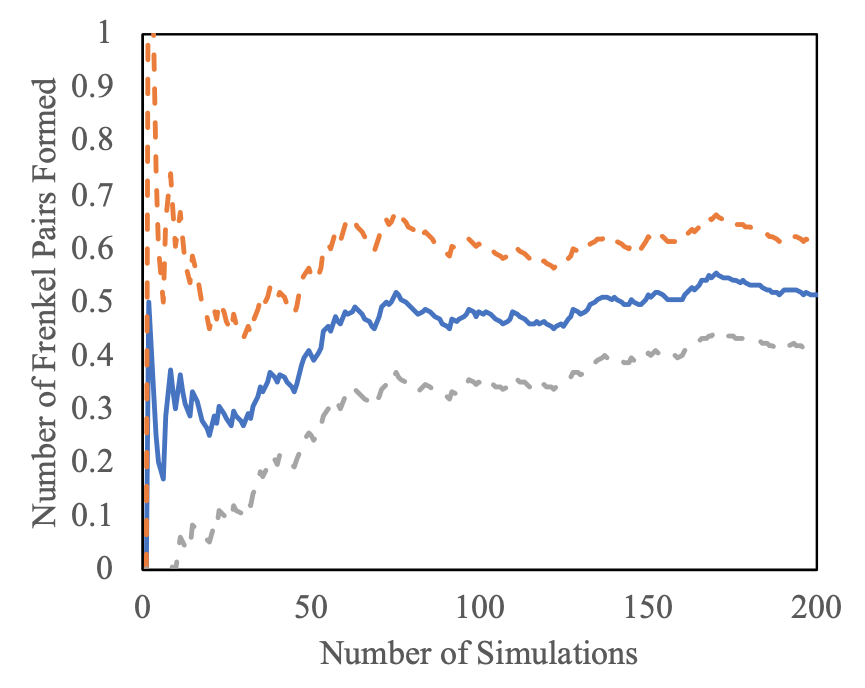
\includegraphics[width=0.6\linewidth]{converge.png}
	\caption{\DIFaddFL{The number of Frenkel pairs as a function of the number of simulations. Twice the standard error of the mean is shown as dashed lines above and below the running average.}}
	\label{fig:converge}
\end{figure}

\FloatBarrier

\DIFaddend Atomic positions were output at various times throughout the simulation in order to accurately investigate all three definitions of the \DIFdelbegin \DIFdel{threshold }\DIFdelend displacement energy. For the first \DIFdelbegin \DIFdel{definition (generation of a Frenkel pair), the Voronoi package within the LAMMPS code \cite{lammps,voro} was utilized. This package creates a Voronoi tesselation at an initial stage and determines if additional atoms are present in the cell (or atoms have left the cell) at the end of the simulation, allowing for a direct way to determine vacancies and interstitials. For the second and third definitions (displacement of PKA off initial lattice siteand permanent displacement off initial lattice site}\DIFdelend \DIFaddbegin \DIFadd{and the second definitions of E$_d$ (probability PKA is displaced from its lattice site, probability of permanently displacing atoms}\DIFaddend ), atomic positions were output once the system reached a thermal state, indicating the end of the thermal spike. It should be noted why atomic positions were output immediately after the return to a thermal state and not at the end of the simulation. Oxygen interstitials diffuse rapidly within these systems, and when one is trying to determine the number of atoms that have been displaced in a system, rapid O interstitial diffusion will artificially inflate this number \DIFdelbegin \DIFdel{, }\DIFdelend due to dumbbell diffusion moving atoms in a chain-like fashion \DIFdelbegin \DIFdel{and self-healing of O interstitials }\DIFdelend \cite{ajay}. Thus, in order to obtain the number of displaced atoms due solely to the damage cascade, systems are quenched immediately following the dissipation of the thermal spike. The specification for the determination of a thermal state is when the sum of excess kinetic energy \DIFdelbegin \DIFdel{, $\sum (KE-1 eV)$, of all atoms above 1 eV }\DIFdelend \DIFaddbegin \DIFadd{(KE$_{xs}$), defined by equation \ref{eq:excess}, }\DIFaddend is less than 5 eV\DIFdelbegin \DIFdel{. In systems with higher energy PKAs, there are approximately 5x more atoms, thus the criterion was increased from 5 eV to 25 eV}\DIFdelend \DIFaddbegin \DIFadd{,
}

\begin{equation}
\DIFadd{\label{eq:excess}
KE_{xs} = \sum_i (KE_i - 1 eV)
}\end{equation}

\DIFadd{where KE$_i$ is the kinetic energy of atom $i$, and KE$_{xs}$ is summed over all atoms}\DIFaddend . These specifications are sufficiently strict to ensure that the PKA energy spike has dissipated. Figure \ref{fig:KE} shows the total excess kinetic energy of atoms above 1 eV as a function of time following the introduction of the PKA. The thermal state is reached \DIFdelbegin \DIFdel{around time step 3}\DIFdelend \DIFaddbegin \DIFadd{at a time of 0.25 ps}\DIFaddend , \DIFdelbegin \DIFdel{500 (0.175 ps) }\DIFdelend where the sum of excess kinetic energy of all particles above 1 eV was \DIFdelbegin \DIFdel{equal to }\DIFdelend \DIFaddbegin \DIFadd{less than }\DIFaddend 5 eV. The figure is made from \DIFdelbegin \DIFdel{an arbitrary run in which the PKA was }\DIFdelend a 50 eV \DIFdelbegin \DIFdel{uranium atom}\DIFdelend \DIFaddbegin \DIFadd{U PKA in a random direction with the Basak potential}\DIFaddend , hence the initial energy of approximately 50 eV.

\DIFdelbegin %DIFDELCMD < \begin{figure}[H]
%DIFDELCMD < %%%
\DIFdelendFL \DIFaddbeginFL \begin{figure}[h]
\DIFaddendFL \centering
	\DIFdelbeginFL %DIFDELCMD < 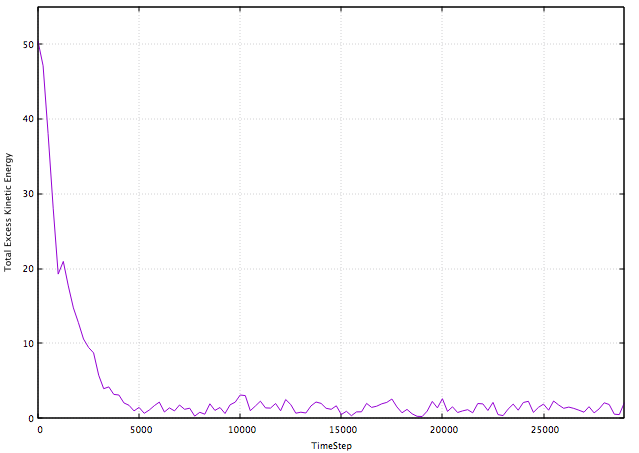
\includegraphics[width=0.6\linewidth]{ETN.png}
%DIFDELCMD < 	%%%
\DIFdelendFL \DIFaddbeginFL 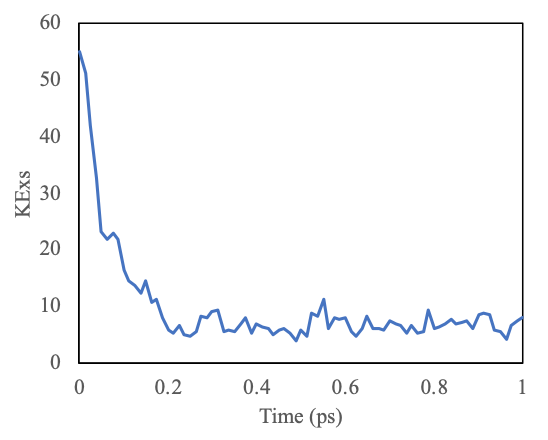
\includegraphics[width=0.6\linewidth]{KExs.png}
	\DIFaddendFL \caption{Total \DIFdelbeginFL \DIFdelFL{Excess }\DIFdelendFL \DIFaddbeginFL \DIFaddFL{excess }\DIFaddendFL kinetic energy for all atoms above 1 eV versus time following the introduction of \DIFdelbeginFL \DIFdelFL{the }\DIFdelendFL \DIFaddbeginFL \DIFaddFL{a }\DIFaddendFL PKA.}
	\label{fig:KE}
\end{figure}

\DIFdelbegin \section{\DIFdel{Results}}
%DIFAUXCMD
\addtocounter{section}{-1}%DIFAUXCMD
\DIFdelend \DIFaddbegin \FloatBarrier
\DIFaddend 

\DIFdelbegin \subsection{\DIFdel{Probability of Frenkel pair formation}}
%DIFAUXCMD
\addtocounter{subsection}{-1}%DIFAUXCMD
\DIFdelend \DIFaddbegin \DIFadd{For the third definition of E$_d$ (generation of a Frenkel pair), the Voronoi package within the LAMMPS code \cite{lammps,voro} was utilized. This package creates a Voronoi tessellation at an initial stage and determines if additional atoms are present in the cell (or atoms have left the cell) at the end of the simulation, allowing for a direct way to determine vacancies and interstitials.
}\DIFaddend 

\DIFdelbegin \DIFdel{\hspace{5mm}
}%DIFDELCMD < 

%DIFDELCMD < %%%
\DIFdel{The probability of Frenkel pair formation as a function of energy for U PKAs is shown in Fig. \ref{fig:fpu}. Probabilities are observed to be zero up to approximately 25 eV for all interatomic potentials and directions. Above 20 eV, probabilities become non-zero and there is a clear directional dependence in the probability curves. The }%DIFDELCMD < [%%%
\DIFdel{214}%DIFDELCMD < ] %%%
\DIFdel{direction consistently exhibits the lowest probability for Frenkel pairformation for all three potentials, while the }%DIFDELCMD < [%%%
\DIFdel{130}%DIFDELCMD < ] %%%
\DIFdel{and }%DIFDELCMD < [%%%
\DIFdel{141}%DIFDELCMD < ] %%%
\DIFdel{directions consistently have the highest probability of Frenkel pair formation. Thus, it is easiest to generate defects from PKAs in the }%DIFDELCMD < [%%%
\DIFdel{130}%DIFDELCMD < ] %%%
\DIFdel{and }%DIFDELCMD < [%%%
\DIFdel{141}%DIFDELCMD < ] %%%
\DIFdel{directions and most difficult to generate defects for PKAs in the }%DIFDELCMD < [%%%
\DIFdel{214}%DIFDELCMD < ] %%%
\DIFdel{direction. Generally, excellent agreement is observed between the potentials. Utilizing the definition of $E_d$ as the lowest energy at which defect formation occurs, the displacement energy for uranium PKAs ($E_d [U]$) is 30 eV for the Basak and Yakub potentials, and 25 eV for the Yamada potential.
This is substantially lower than the experimentally reported value of 40 eV \cite{soullard1977,soullard1985}.
}%DIFDELCMD < 

%DIFDELCMD < %%%
\DIFdel{It can often be valuable to generate an average probability curve and analyze the median of this curve (the point where the probability becomes greater than 0.5). This value for $E_{d}$ is not a quantity directly comparable to experiment, but is likely the more appropriate value for usage in the NRT equation \cite{nordlund2006, beelertde}. Thus, the results for the six PKA directions are linearly averaged to create a single probability curve for Frenkel pair formation }\DIFdelend \DIFaddbegin \DIFadd{For each definition of E$_d$, a distribution is generated for the probability }\DIFaddend as a function of PKA energy. \DIFdelbegin \DIFdel{The median value for $E_d [U]$ is 54 eV for Basak, 54 eV for Yakub, and 55.5 eV for Yamada. Interestingly, this interpretation for $E_{d}$ compares very favorably to the computational studies of Meis \cite{meis2005}. It should be noted that given this limited set of PKA directions, a true crystallographically averaged Frenkel pairformation probability curve would likely be different in nature. However, this simplified exercise can still provide a valuable approximation for the average behavior of U PKAs in the $UO_{2}$ system.
}%DIFDELCMD < 

%DIFDELCMD < \begin{figure*}[h]
%DIFDELCMD <  \centering
%DIFDELCMD <  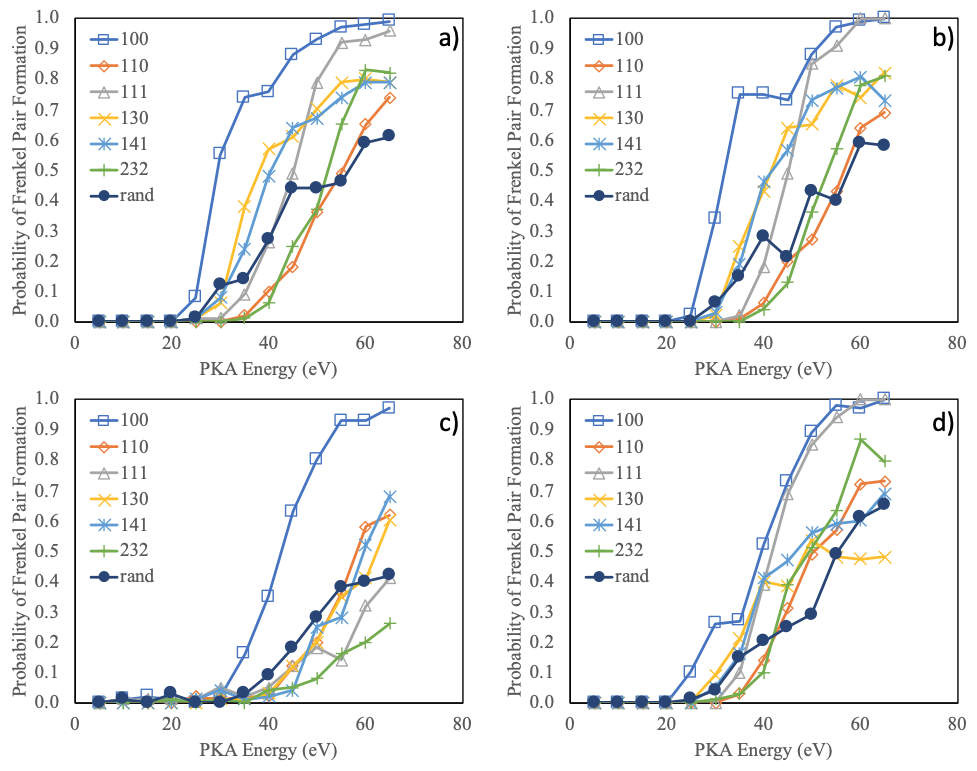
\includegraphics[width=1.0\textwidth]{FP_U.png}
%DIFDELCMD <  %%%
%DIFDELCMD < \caption{%
{%DIFAUXCMD
\DIFdelFL{Probability of Frenkel pair formation as a function of PKA energy in $UO_2$ due to uranium PKAs in the }%DIFDELCMD < [%%%
\DIFdelFL{110}%DIFDELCMD < ]%%%
\DIFdelFL{, }%DIFDELCMD < [%%%
\DIFdelFL{130}%DIFDELCMD < ]%%%
\DIFdelFL{, }%DIFDELCMD < [%%%
\DIFdelFL{141}%DIFDELCMD < ]%%%
\DIFdelFL{, }%DIFDELCMD < [%%%
\DIFdelFL{214}%DIFDELCMD < ]%%%
\DIFdelFL{, }%DIFDELCMD < [%%%
\DIFdelFL{232}%DIFDELCMD < ] %%%
\DIFdelFL{and }%DIFDELCMD < [%%%
\DIFdelFL{313}%DIFDELCMD < ] %%%
\DIFdelFL{directions for the a) Basak, b) Yakub and c) Yamada potentials.  }}
 %DIFAUXCMD
%DIFDELCMD < \label{fig:fpu}
%DIFDELCMD < \end{figure*}
%DIFDELCMD < 

%DIFDELCMD < %%%
\DIFdel{The probability of }\DIFdelend \DIFaddbegin \DIFadd{In order to extract a value for the E$_d$ for each of these distributions, E$_d$ is determined as the energy at which the probability is equal to, or greater than, 0.5. This indicates that it is likely to either displace a PKA from it lattice site, permanently displace an atom, or create a }\DIFaddend Frenkel \DIFdelbegin \DIFdel{pair formation }\DIFdelend \DIFaddbegin \DIFadd{pair, respectively. Additionally, for the second and third definitions of E$_d$, the \textit{total number} of displaced atoms and the \textit{total number} of Frenkel pairs produced are determined }\DIFaddend as a function of \DIFdelbegin \DIFdel{energy for O PKAs is shown in Fig. \ref{fig:fpo}. Probabilities are consistently below 0.1 for all PKA energies investigated in this range. Oxygen PKAs at these low energies are unable to transfer sufficient energy to displace uranium atoms, thus only O defects can be formed. Albeit very minimal, probabilities do become non-zero near a PKA energy of 20 eV.
Utilizing the definition of $E_d$ as the lowest energy at which defect formation occurs, the displacement energy for oxygen PKAs ($E_d [O]$) is is 20 eV for the Basak potential and 30 eV for both the Yakub and Yamada potentials. This can be viewed as in concordance with the experimentally observed $E_d [O]$ of 20 eV \cite{soullard1977,soullard1985}. No observable directional dependence can be elucidated from these results, as the statistical noise from this sample is equal to the magnitude of the probabilities. Similarly, comparisons of potentials in untenable due to the rare Frenkel pair formation events.
}\DIFdelend \DIFaddbegin \DIFadd{PKA energy. A secondary value of E$_d$ is defined as when it is likely to displace one atom or to create one Frenkel pair. This secondary formalism of E$_d$ may or may not necessarily match the value for the primary formalism. Although both characterizations will be investigated, only the first formalism based on probabilities will be utilized for comparisons among different definitions of E$_d$.
}\DIFaddend 

\DIFdelbegin \DIFdel{Given that the probability of Frenkel pair formation does not exceed 0.1 for the range of PKA energies, }\DIFdelend \DIFaddbegin \DIFadd{A discussion on the meaning of }\DIFaddend the \DIFdelbegin \DIFdel{construction of a directionally-averaged probability curve (in order to obtain the PKA energy where the probability becomes greater than 0.5) is meaningless}\DIFdelend \DIFaddbegin \DIFadd{terms permanent and stable needs to be undertaken. These terms are relative and defined in this manuscript on a picosecond timescale. The permanent displacement of an atom from its lattice site means that the atom has been moved from its original lattice site and exists at a different lattice site at the end of the thermal spike. A stable Frenkel pair means that a Frenkel pair exists at the end of the simulation (after 5.5 ps at 1500 K). The authors are aware that additional recombination, defect clustering, and migration is possible. However, given the constrains of molecular dynamics timescales, this work provides a reasonable result for the defect population produced from cascades that can then be utilized in higher timescale modeling methodologies such as kinetic Monte Carlo and cluster dynamics to investigate further defect evolution. A more complete discussion on the investigation of Frenkel pair recombination distance and lifetime was undertaken by Van Brutzel \cite{vanbrutzel2008} and can be consulted for extrapolation of these results}\DIFaddend .

\DIFdelbegin %DIFDELCMD < \begin{figure*}[h]
%DIFDELCMD <  \centering
%DIFDELCMD <  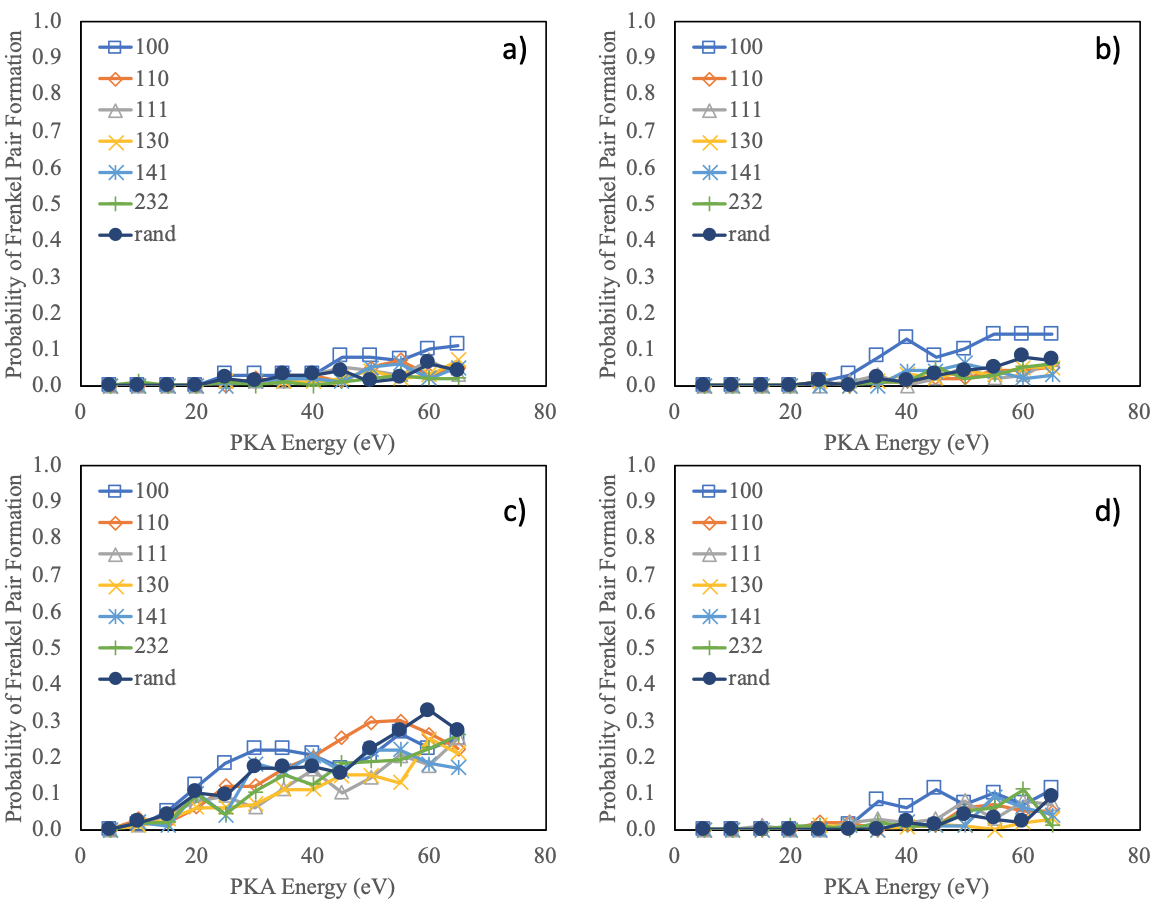
\includegraphics[width=1.0\textwidth]{FP_O.png}
%DIFDELCMD <  %%%
%DIFDELCMD < \caption{%
{%DIFAUXCMD
\DIFdelFL{Probability of Frenkel pair formation as a function of PKA energy in $UO_2$ due to oxygen PKAs in the }%DIFDELCMD < [%%%
\DIFdelFL{110}%DIFDELCMD < ]%%%
\DIFdelFL{, }%DIFDELCMD < [%%%
\DIFdelFL{130}%DIFDELCMD < ]%%%
\DIFdelFL{, }%DIFDELCMD < [%%%
\DIFdelFL{141}%DIFDELCMD < ]%%%
\DIFdelFL{, }%DIFDELCMD < [%%%
\DIFdelFL{214}%DIFDELCMD < ]%%%
\DIFdelFL{, }%DIFDELCMD < [%%%
\DIFdelFL{232}%DIFDELCMD < ] %%%
\DIFdelFL{and }%DIFDELCMD < [%%%
\DIFdelFL{313}%DIFDELCMD < ] %%%
\DIFdelFL{directions for the a) Basak, b) Yakub and c) Yamada potentials.  }}
 %DIFAUXCMD
%DIFDELCMD < \label{fig:fpo}
%DIFDELCMD < \end{figure*}
%DIFDELCMD < 

%DIFDELCMD < %%%
\DIFdelend \FloatBarrier

\DIFaddbegin \section{\DIFadd{Results}}

\DIFaddend \subsection{Probability of \DIFdelbegin \DIFdel{lattice site }\DIFdelend \DIFaddbegin \DIFadd{PKA }\DIFaddend displacement}\DIFdelbegin \DIFdel{\hspace{5mm}
}\DIFdelend \DIFaddbegin \label{sect1}

\subsubsection{\DIFadd{Uranium PKA}}

\DIFaddend The probability of the PKA leaving its lattice site in \DIFdelbegin \DIFdel{$UO_2$ }\DIFdelend \DIFaddbegin \DIFadd{UO$_2$ }\DIFaddend for uranium PKAs is shown in Fig. \DIFdelbegin \DIFdel{\ref{fig:latu}}\DIFdelend \DIFaddbegin \DIFadd{\ref{fig:pkau} for all sets of PKA directions and all four interatomic potentials}\DIFaddend . It is observed that U PKAs can be displaced from their lattice site at an energy as low as \DIFdelbegin \DIFdel{15 }\DIFdelend \DIFaddbegin \DIFadd{10 }\DIFaddend eV. It should be emphasized that this does not denote the generation of a defect or a permanent displacement of an atom off of its lattice site, simply that the PKA achieved a maximum displacement sufficient to be classified as no longer on its original lattice site. \DIFdelbegin \DIFdel{It makes qualitative sense, provided the nature of the definition, that the observed energies for non-zero probabilities in Fig. \ref{fig:latu} are much lower than in Fig. \ref{fig:fpu}. The highest probabilities }\DIFdelend \DIFaddbegin \DIFadd{The highest probability }\DIFaddend of PKA displacement \DIFdelbegin \DIFdel{are }\DIFdelend \DIFaddbegin \DIFadd{is }\DIFaddend observed for the [\DIFdelbegin \DIFdel{130}%DIFDELCMD < ] %%%
\DIFdel{and }%DIFDELCMD < [%%%
\DIFdel{141}%DIFDELCMD < ] %%%
\DIFdel{directions, similar to the results in Fig. \ref{fig:latu}. These directions show a }\DIFdelend 100\DIFdelbegin %DIFDELCMD < {%%%
\DIFdel{\%}%DIFDELCMD < } %%%
\DIFdel{likelihood of PKA displacement above an energy of 20 eV. Interestingly, }\DIFdelend \DIFaddbegin ] \DIFadd{direction, while the lowest probability is observed for }\DIFaddend the [110] direction\DIFdelbegin \DIFdel{exhibits the lowest probability of PKA displacement. Thus one can conclude from Fig. \ref{fig:fpu} and Fig. \ref{fig:latu} that although it is more difficult to displace an U atom from its lattice site in the }\DIFdelend \DIFaddbegin \DIFadd{. This relationship is present for all potentials analyzed. It is likely that this is due to the proximity of the nearest neighbor in the specific PKA direction. In the }\DIFaddend [\DIFdelbegin \DIFdel{110}\DIFdelend \DIFaddbegin \DIFadd{100}\DIFaddend ] direction, \DIFdelbegin \DIFdel{there is a significant probability of that atom forming a stable Frenkel pair. This is not the case for the }\DIFdelend \DIFaddbegin \DIFadd{the nearest neighbor is at a distance of one full lattice parameter, while in the }\DIFaddend [\DIFdelbegin \DIFdel{214}\DIFdelend \DIFaddbegin \DIFadd{110}\DIFaddend ] direction, \DIFdelbegin \DIFdel{where is it moderately easy to displace an atom from its lattice site, but that atom is very unlikely to form a stable Frenkel pair. Excellent agreement is shown across all three potentials for the magnitude and the relative probabilities of PKA directions. Linearly averaging over the set }\DIFdelend \DIFaddbegin \DIFadd{the nearest neighbor is only at a distance of $\sqrt{2}$/2 times the lattice parameter, which is a significantly closer neighbor. Such a variability in the local environment produces such changes in PKA displacement probability. For the random set of directions, the PKA has a greater than 90\% probability of being displaced for PKA energies of at least 35 eV for all potentials except the Morelon, which requires 50 eV of kinetic energy to yield a 90\% probability of displacing the PKA. Utilizing the random set of directions as approximating average behavior and taking a probability }\DIFaddend of \DIFdelbegin \DIFdel{PKA directionsin Fig. \ref{fig:latu} allows for the creation of a single probability curve for PKA lattice site displacement as a function of PKA energy. The single probability curve enables us to obtain the PKA energy where it is probable to displace a U atom from its lattice site. This formalism of $E_d [U]$ is 23.1 eV , 25.5 eV and 24.6 eV }\DIFdelend \DIFaddbegin \DIFadd{50\% to represent E$_d$, the value of E$_d$ for U PKAs (E$_d$}[\DIFadd{U}]\DIFadd{) is determined to be 25 eV }\DIFaddend for the Basak \DIFdelbegin \DIFdel{, Yakub and Yamada potentials, respectively}\DIFdelend \DIFaddbegin \DIFadd{and Yakub potentials, 35 eV for the Morelon potential and 20 eV for the Cooper potential}\DIFaddend .

\begin{figure*}[h]
 \centering
 \DIFdelbeginFL %DIFDELCMD < 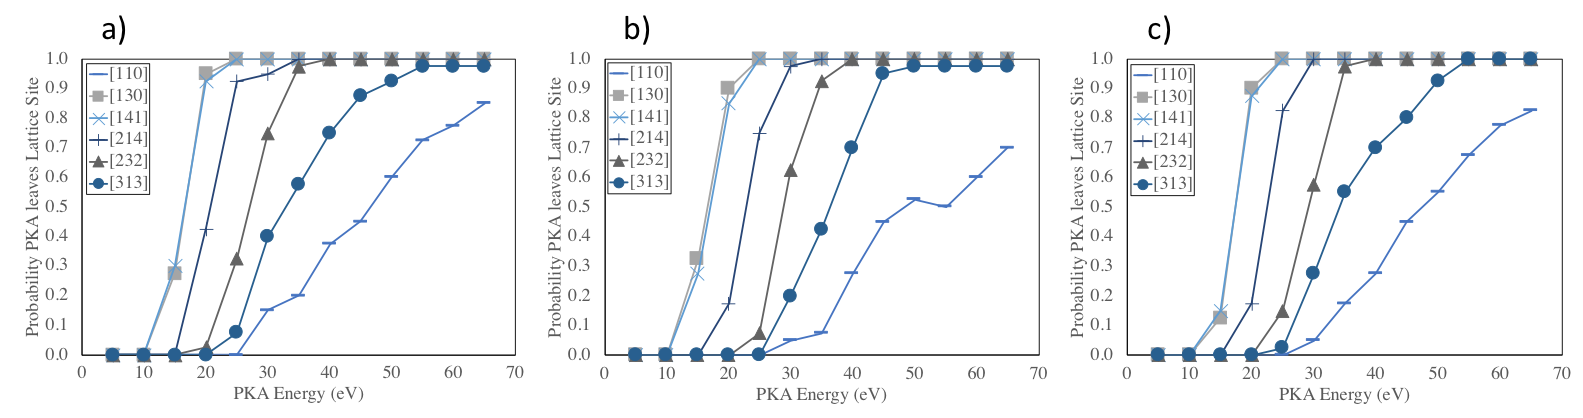
\includegraphics[width=1.0\textwidth]{lat_U.png}
%DIFDELCMD <  %%%
\DIFdelendFL \DIFaddbeginFL 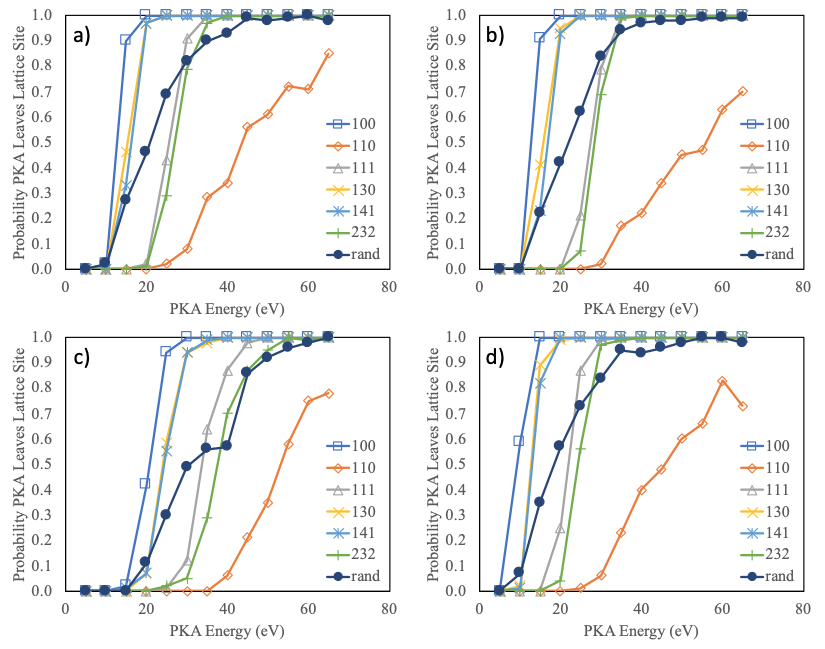
\includegraphics[width=1.0\textwidth]{pka_Upka.png}
 \DIFaddendFL \caption{Probability of PKA leaving lattice site in \DIFdelbeginFL \DIFdelFL{$UO_2$ }\DIFdelendFL \DIFaddbeginFL \DIFaddFL{UO$_2$ }\DIFaddendFL for uranium PKAs in the [\DIFaddbeginFL \DIFaddFL{100}]\DIFaddFL{, }[\DIFaddendFL 110], [\DIFdelbeginFL \DIFdelFL{130}\DIFdelendFL \DIFaddbeginFL \DIFaddFL{111}\DIFaddendFL ], [\DIFdelbeginFL \DIFdelFL{141}\DIFdelendFL \DIFaddbeginFL \DIFaddFL{130}\DIFaddendFL ], [\DIFdelbeginFL \DIFdelFL{214}\DIFdelendFL \DIFaddbeginFL \DIFaddFL{141}\DIFaddendFL ], [232] and \DIFdelbeginFL %DIFDELCMD < [%%%
\DIFdelFL{313}%DIFDELCMD < ] %%%
\DIFdelendFL \DIFaddbeginFL \DIFaddFL{random }\DIFaddendFL directions for the a) Basak, b) Yakub\DIFdelbeginFL \DIFdelFL{and }\DIFdelendFL \DIFaddbeginFL \DIFaddFL{, }\DIFaddendFL c) \DIFdelbeginFL \DIFdelFL{Yamada }\DIFdelendFL \DIFaddbeginFL \DIFaddFL{Morelon, and d) Cooper }\DIFaddendFL potentials. }
 \DIFdelbeginFL %DIFDELCMD < \label{fig:latu}
%DIFDELCMD < %%%
\DIFdelendFL \DIFaddbeginFL \label{fig:pkau}
\DIFaddendFL \end{figure*}

\DIFaddbegin \FloatBarrier

\subsubsection{\DIFadd{Oxygen PKA}}

\DIFaddend The probability of the PKA leaving its lattice site in \DIFdelbegin \DIFdel{$UO_2$ }\DIFdelend \DIFaddbegin \DIFadd{UO$_2$ }\DIFaddend for oxygen PKAs is shown in Fig. \DIFdelbegin \DIFdel{\ref{fig:lato}}\DIFdelend \DIFaddbegin \DIFadd{\ref{fig:pkao} for all sets of PKA directions and all four interatomic potentials}\DIFaddend . It is observed that O PKAs can be displaced from their lattice site at an energy as low as 10 eV. \DIFdelbegin \DIFdel{The highest probability of PKA displacement is observed }\DIFdelend \DIFaddbegin \DIFadd{Analyzing the different directions, it is observed that the highest probability is }\DIFaddend for the [110] direction\DIFaddbegin \DIFadd{, }\DIFaddend while the lowest probability \DIFdelbegin \DIFdel{of PKA displacement is observed }\DIFdelend \DIFaddbegin \DIFadd{is }\DIFaddend for the [\DIFdelbegin \DIFdel{232}\DIFdelend \DIFaddbegin \DIFadd{100}\DIFaddend ] direction. This \DIFdelbegin \DIFdel{directional dependence is consistent over the three interatomic potentials. However, there is a noticeable difference in the magnitude of the displacement probabilities for the Yamada potential when compared to the }\DIFdelend \DIFaddbegin \DIFadd{is in direct contrast to the U PKAs, but perfectly corresponds to nearest neighbor distances in the crystal structure. Oxygen atoms are organized on a simple cubic sublattice inside the U face-centered cubic sublattice, comprising the UO$_2$ fluorite structure. As such, the closest nearest neighbor distance for O atoms is along the }[\DIFadd{100}] \DIFadd{direction, which exhibits the lowest probability of PKA displacement. Utilizing the random set of directions as approximating average behavior and taking a probability of 0.5 to represent E$_d$, the value of E$_d$ for O PKAs (E$_d$}[\DIFadd{O}]\DIFadd{) is determined to be 15 eV for the }\DIFaddend Basak and Yakub potentials \DIFdelbegin \DIFdel{. The PKA displacement probability curves are shifted to the right for the Yamada potential, suggesting a greater difficulty of moving the O PKA from its lattice site. The data }\DIFdelend \DIFaddbegin \DIFadd{and 10 eV for the Morelon and Cooper potentials.
}

\begin{figure*}[h]
 \centering
 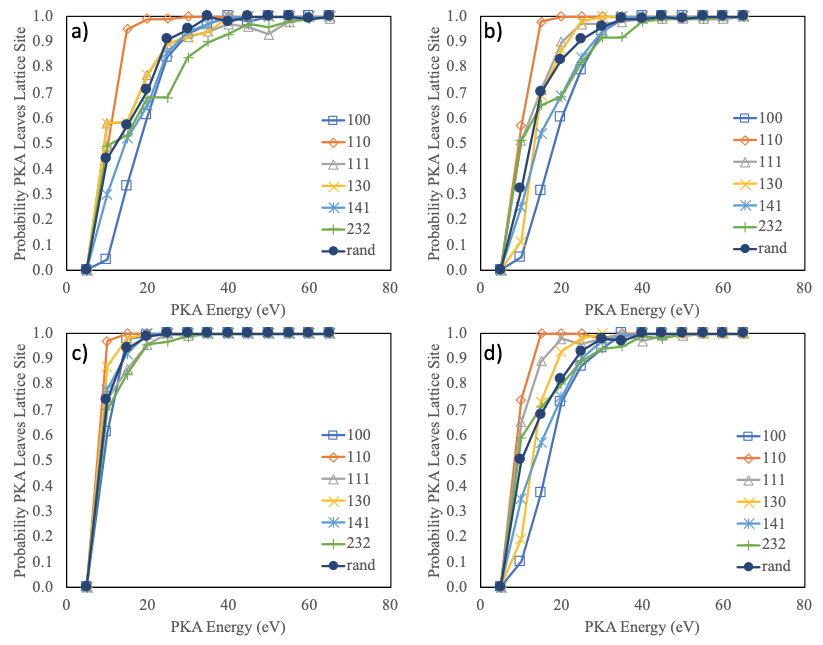
\includegraphics[width=1.0\textwidth]{pka_Opka.png}
 \caption{\DIFaddFL{Probability of PKA leaving lattice site in UO$_2$ for oxygen PKAs in the }[\DIFaddFL{100}]\DIFaddFL{, }[\DIFaddFL{110}]\DIFaddFL{, }[\DIFaddFL{111}]\DIFaddFL{, }[\DIFaddFL{130}]\DIFaddFL{, }[\DIFaddFL{141}]\DIFaddFL{, }[\DIFaddFL{232}] \DIFaddFL{and random directions for the a) Basak, b) Yakub, c) Morelon, and d) Cooper potentials.}}
 \label{fig:pkao}
\end{figure*}

\FloatBarrier

\subsection{\DIFadd{Permanent displacement of atoms}}\label{sect2}

\subsubsection{\DIFadd{Uranium PKA}}

\DIFadd{The probability of the U PKA causing permanent displacement of atoms is shown }\DIFaddend in Fig. \DIFdelbegin \DIFdel{\ref{fig:lato} is utilized to construct a single probability curve for PKA lattice site displacement as a function of PKA energy. Taking the median of this data, the $E_d [O]$ is 14.6 eV , 16.4 eV and 19.5 eV }\DIFdelend \DIFaddbegin \DIFadd{\ref{fig:dispU} for all sets of PKA directions and all four interatomic potentials. It is observed that U PKAs begin to permanently displace atoms at 15 eV }\DIFaddend for the Basak, Yakub and \DIFdelbegin \DIFdel{Yamada potentials , respectively. This more clearly illustrates the shift right of the data of the Yamada potential. }\DIFdelend \DIFaddbegin \DIFadd{Cooper potentials and at 10 eV for the Morelon potential. Similar crystallographic relatedness is observed to the results in Fig. \ref{fig:pkau}, where the }[\DIFadd{110}] \DIFadd{direction generally displays the lowest probability of displacement and the }[\DIFadd{100}[ \DIFadd{generally displays the highest probability of displacement. The value of E$_d$}[\DIFadd{U}] \DIFadd{is determined to be 45 eV for all four interatomic potentials investigated.
}\DIFaddend 

\begin{figure*}[h]
 \centering
 \DIFdelbeginFL %DIFDELCMD < 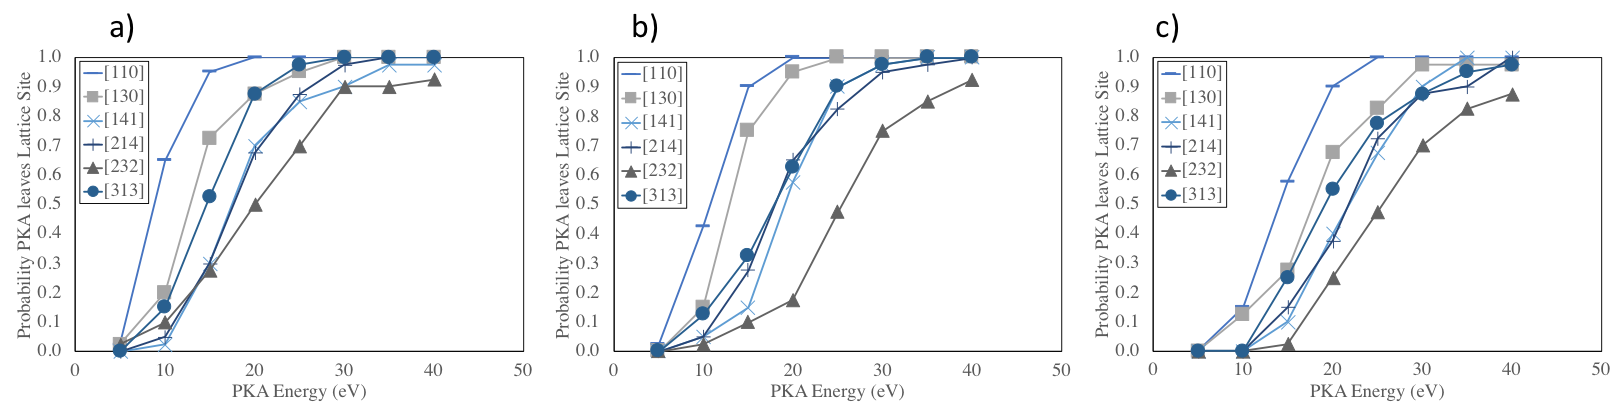
\includegraphics[width=1.0\textwidth]{lat_O.png}
%DIFDELCMD <  %%%
\DIFdelendFL \DIFaddbeginFL 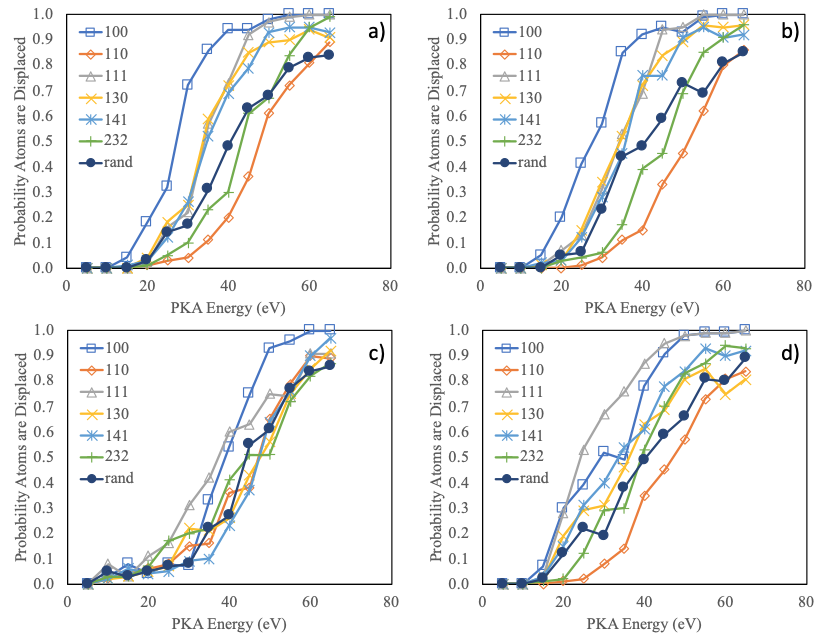
\includegraphics[width=1.0\textwidth]{dispU.png}
 \DIFaddendFL \caption{Probability of \DIFaddbeginFL \DIFaddFL{U }\DIFaddendFL PKA \DIFdelbeginFL \DIFdelFL{leaving lattice site }\DIFdelendFL \DIFaddbeginFL \DIFaddFL{permanently displacing atoms }\DIFaddendFL in \DIFdelbeginFL \DIFdelFL{$UO_2$ }\DIFdelendFL \DIFaddbeginFL \DIFaddFL{UO$_2$ }\DIFaddendFL for \DIFdelbeginFL \DIFdelFL{oxygen }\DIFdelendFL PKAs in the [\DIFaddbeginFL \DIFaddFL{100}]\DIFaddFL{, }[\DIFaddendFL 110], [\DIFdelbeginFL \DIFdelFL{130}\DIFdelendFL \DIFaddbeginFL \DIFaddFL{111}\DIFaddendFL ], [\DIFdelbeginFL \DIFdelFL{141}\DIFdelendFL \DIFaddbeginFL \DIFaddFL{130}\DIFaddendFL ], [\DIFdelbeginFL \DIFdelFL{214}\DIFdelendFL \DIFaddbeginFL \DIFaddFL{141}\DIFaddendFL ], [232] and \DIFdelbeginFL %DIFDELCMD < [%%%
\DIFdelFL{313}%DIFDELCMD < ] %%%
\DIFdelendFL \DIFaddbeginFL \DIFaddFL{random }\DIFaddendFL directions for the a) Basak, b) Yakub\DIFdelbeginFL \DIFdelFL{and }\DIFdelendFL \DIFaddbeginFL \DIFaddFL{, }\DIFaddendFL c) \DIFdelbeginFL \DIFdelFL{Yamada }\DIFdelendFL \DIFaddbeginFL \DIFaddFL{Morelon, and d) Cooper }\DIFaddendFL potentials.}
 \DIFdelbeginFL %DIFDELCMD < \label{fig:lato}
%DIFDELCMD < %%%
\DIFdelendFL \DIFaddbeginFL \label{fig:dispU}
\DIFaddendFL \end{figure*}

\FloatBarrier

\DIFdelbegin \subsection{\DIFdel{Permanent displacement of atoms}}
%DIFAUXCMD
\addtocounter{subsection}{-1}%DIFAUXCMD
\subsubsection{\DIFdel{Displaced oxygen atoms}}
%DIFAUXCMD
\addtocounter{subsubsection}{-1}%DIFAUXCMD
\DIFdel{\hspace{5mm}
}%DIFDELCMD < 

%DIFDELCMD < %%%
\DIFdel{The average number of oxygen atoms permanently displaced per U PKA as a function of PKA energy is shown in Fig. \ref{fig:dispou}. Permanent displacement of O }\DIFdelend \DIFaddbegin \DIFadd{In addition to the probability of displacing atoms, the total number and type of }\DIFaddend atoms \DIFdelbegin \DIFdel{begins at a PKA energy of approximately 20 eV. Although there exist directional dependencies for each individual potential, a general trend for high or low displacement directions across all potentials is not observable. A clear observation is the distinct differences between the three potentials. The Basak and Yamada potentials display similar behavior, while the Yamada potential predicts significantly more displaced O atoms for a U PKA of a given energy. To more clearly illustrate this phenomenon, the results for each potential are averaged over the investigated directions . At a U PKA energy of 60 eV, the directionally-averaged number of displaced O atoms per UPKA is 4.5}\DIFdelend \DIFaddbegin \DIFadd{displaced provides information relevant to the effects of radiation damage. Fig. \ref{fig:dispall} displays the total number of atoms displaced, along with the individual number of U and O atoms displaced as a function of PKA energy for U PKAs. For all interatomic potentials}\DIFaddend , \DIFdelbegin \DIFdel{3.4 and 8.1 }\DIFdelend \DIFaddbegin \DIFadd{the majority of the displaced atoms are O atoms, with a ratio of O atoms displaced to U atoms displaced from approximately 4:1 up to 6:1. The total number of atoms displaced follows the same crystallographic trends as the probability that atoms are displaced from Fig. \ref{fig:dispU}. Utilizing the random set of directions to approximate average behavior and utilizing the secondary formalism of E$_d$ (when a PKA displaces on average one atom), the value of E$_d$}[\DIFadd{U}] \DIFadd{is 35 eV }\DIFaddend for the Basak, Yakub and \DIFdelbegin \DIFdel{Yamada potentials , respectively. It should be emphasized that this does not necessarily indicate the generation of a Frenkel pair, but only the permanent displacement of an atom off of its original lattice site. }\DIFdelend \DIFaddbegin \DIFadd{Cooper potentials and 40 eV for the Morelon potential. This formalism of E$_d$, although it investigates the same type of local atomic changes due to a PKA, yields slightly lower values for E$_d$}[\DIFadd{U}] \DIFadd{than for the first formalism extracted from Fig. \ref{fig:dispU}.
}\DIFaddend 

\DIFaddbegin \DIFadd{Finally, it can be observed from Fig. \ref{fig:dispall} the different U PKA energies at which a O atom or a U atom is displaced. O atoms typically begin to be displaced at U PKA energies of 20 eV and U atoms tend to begin to be displaced at U PKA energies of 30 eV. Thus even though the PKA is U, it still requires approximately 10 eV less energy to displace a O atom, than a U atom.
}

\DIFaddend \begin{figure*}[h]
 \centering
 \DIFdelbeginFL %DIFDELCMD < 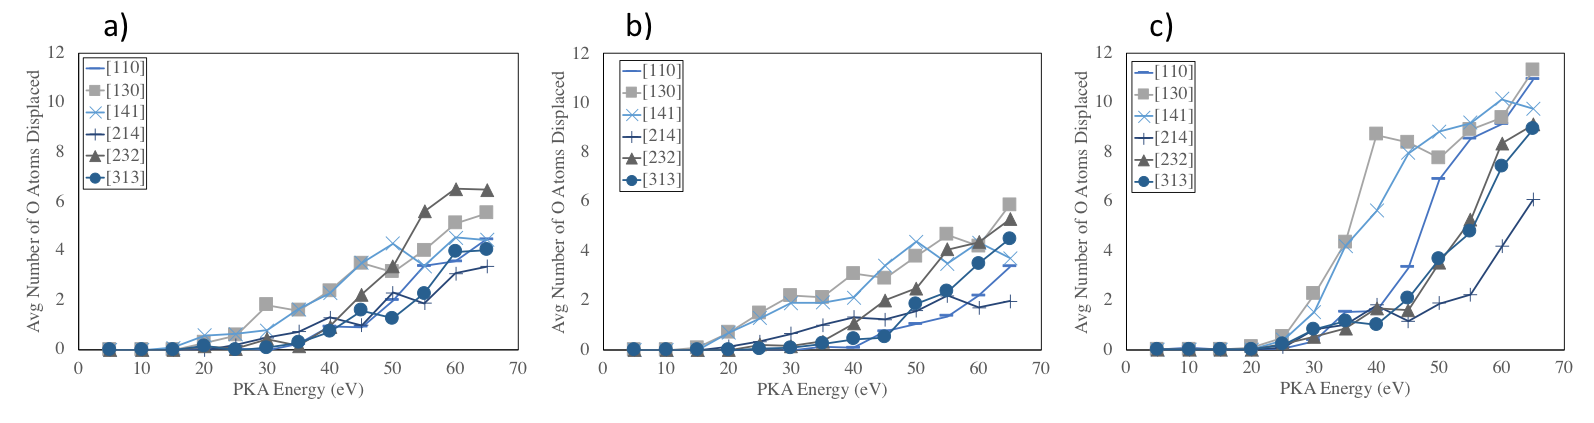
\includegraphics[width=1.0\textwidth]{dispO_U.png}
%DIFDELCMD <  %%%
%DIFDELCMD < \caption{%
{%DIFAUXCMD
\DIFdelFL{Average number of oxygen atoms displaced by a U PKA as a function of PKA energy in $UO_2$ in the }%DIFDELCMD < [%%%
\DIFdelFL{110}%DIFDELCMD < ]%%%
\DIFdelFL{, }%DIFDELCMD < [%%%
\DIFdelFL{130}%DIFDELCMD < ]%%%
\DIFdelFL{, }%DIFDELCMD < [%%%
\DIFdelFL{141}%DIFDELCMD < ]%%%
\DIFdelFL{, }%DIFDELCMD < [%%%
\DIFdelFL{214}%DIFDELCMD < ]%%%
\DIFdelFL{, }%DIFDELCMD < [%%%
\DIFdelFL{232}%DIFDELCMD < ] %%%
\DIFdelFL{and }%DIFDELCMD < [%%%
\DIFdelFL{313}%DIFDELCMD < ] %%%
\DIFdelFL{directions for the a) Basak, b) Yakub and c) Yamada potentials.  }}
 %DIFAUXCMD
%DIFDELCMD < \label{fig:dispou}
%DIFDELCMD < %%%
\DIFdelendFL \DIFaddbeginFL 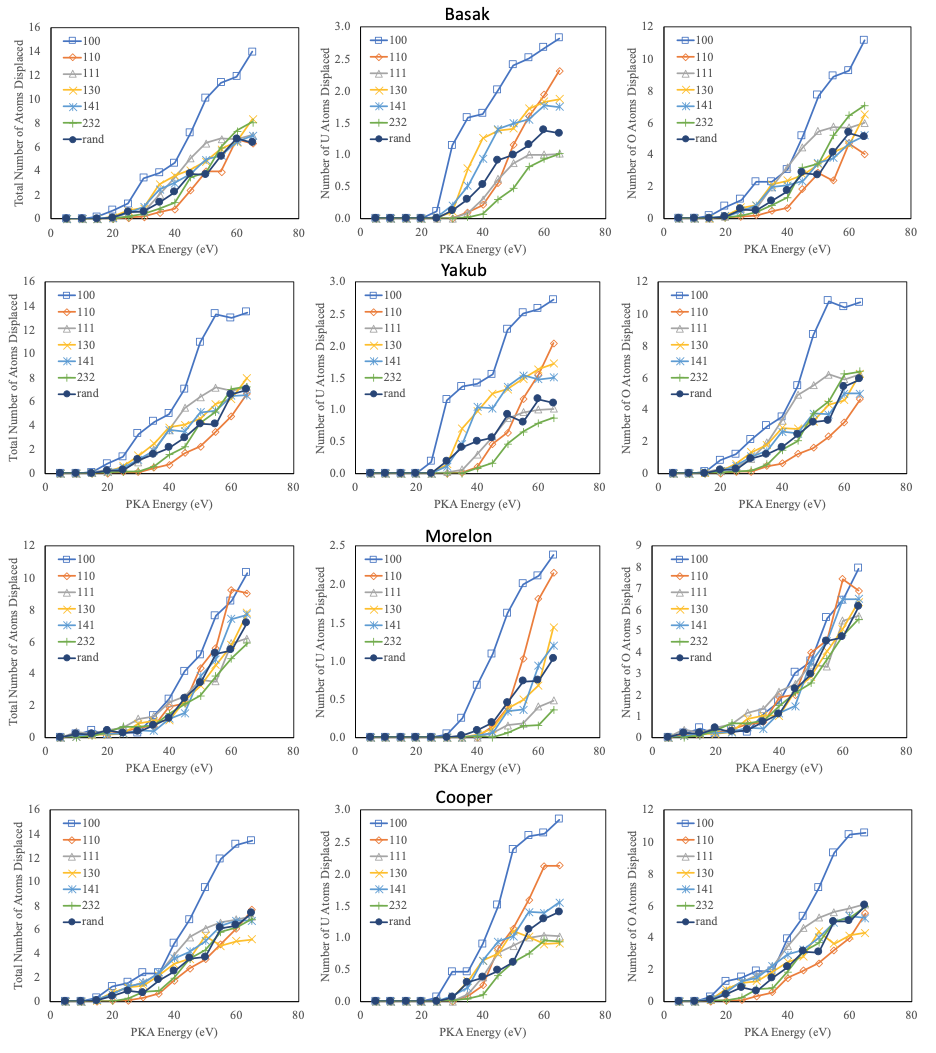
\includegraphics[width=1.0\textwidth]{disp_allU.png}
 \caption{\DIFaddFL{The number of atoms permanently displaced in UO$_2$ by U PKAs in the }[\DIFaddFL{100}]\DIFaddFL{, }[\DIFaddFL{110}]\DIFaddFL{, }[\DIFaddFL{111}]\DIFaddFL{, }[\DIFaddFL{130}]\DIFaddFL{, }[\DIFaddFL{141}]\DIFaddFL{, }[\DIFaddFL{232}] \DIFaddFL{and random directions for the Basak, Yakub, Morelon, and Cooper potentials. The total number of displaced atoms, as well as the number of U and O atoms displaced is displayed.}}
 \label{fig:dispall}
\DIFaddendFL \end{figure*}

\DIFdelbegin \DIFdel{The average number of oxygen atoms permanently displaced per O PKA as a function of PKA energy is shown in Fig. \ref{fig:dispoo}. Permanent displacement of atoms begins at an O PKA energy of approximately 20 }\DIFdelend \DIFaddbegin \FloatBarrier

\subsubsection{\DIFadd{Oxygen PKA}}

\DIFadd{The probability of the O PKA causing permanent displacement of atoms is shown in Fig. \ref{fig:dispO} for all sets of PKA directions and all four interatomic potentials. It is observed that O PKAs begin to permanently displace atoms at approximately 15 }\DIFaddend eV \DIFdelbegin \DIFdel{. It is interesting to note that the minimum required energy to permanently displace an O atomfrom its lattice site is independent of whether the PKA is a U or an O atom.
The }%DIFDELCMD < [%%%
\DIFdel{232}%DIFDELCMD < ] %%%
\DIFdel{direction consistently exhibits the fewest number of oxygen atoms displaced per PKA across all potentials. The }%DIFDELCMD < [%%%
\DIFdel{110}%DIFDELCMD < ] %%%
\DIFdel{O PKA direction leads to the highest number of displaced O atoms }\DIFdelend for the Basak\DIFdelbegin \DIFdel{and Yakub potentials, while no single high displacement direction exists for the Yamada potential. Additionally, the magnitude of the displaced Oatoms is less for the Yamada potentialthan for the Basak and Yakub potentials. The results for each potentialare averaged over the investigated directions.
At }\DIFdelend \DIFaddbegin \DIFadd{, Yakub and Cooper potentials and at 10 eV for the Morelon potential. It is difficult to discern crystallographic variation, as the data are relatively closely bunched. This indicates at minimum a weak dependence upon PKA direction. The value of E$_d$}[\DIFadd{O}] \DIFadd{is determined as 60 eV for the Basak potential, 45 eV for the Yakub and Cooper potentials, and 20 eV for the Morelon potential. This is a wide disparity in the values for E$_d$}[\DIFadd{O}] \DIFadd{that was not present for the definition of E$_d$}[\DIFadd{O}] \DIFadd{in section \ref{sect1}.
}

\begin{figure*}[h]
 \centering
 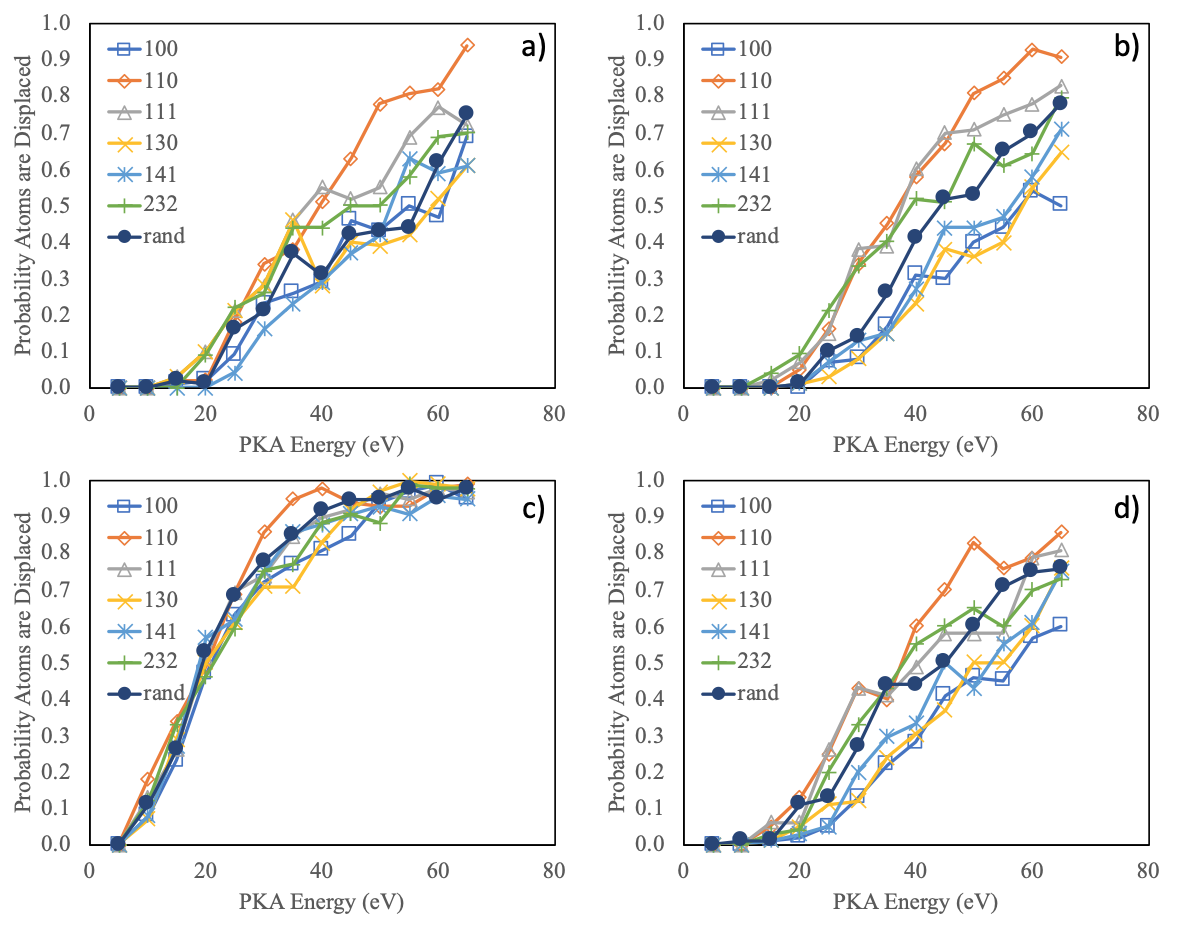
\includegraphics[width=1.0\textwidth]{dispO.png}
 \caption{\DIFaddFL{Probability of O PKA permanently displacing atoms in UO$_2$ for PKAs in the }[\DIFaddFL{100}]\DIFaddFL{, }[\DIFaddFL{110}]\DIFaddFL{, }[\DIFaddFL{111}]\DIFaddFL{, }[\DIFaddFL{130}]\DIFaddFL{, }[\DIFaddFL{141}]\DIFaddFL{, }[\DIFaddFL{232}] \DIFaddFL{and random directions for the a) Basak, b) Yakub, c) Morelon, and d) Cooper potentials.}}
 \label{fig:dispO}
\end{figure*}

\FloatBarrier

\DIFadd{Fig. \ref{fig:dispallO} displays the number of O atoms displaced due to }\DIFaddend an O PKA\DIFdelbegin \DIFdel{energy of 40 eV, the directionally-averaged number of displaced O atoms per O PKA }\DIFdelend \DIFaddbegin \DIFadd{. Oxygen atoms at these energies are not moving rapidly enough to displace U atoms, and as such the number of O atoms displaced in Fig. \ref{fig:dispallO} is also the total number of atoms displaced. There is a general linear trend for the number of O atoms displaced as a function of PKA energy over this energy range, with the interatomic potential determining the slope of the linear relationship. It should be emphasized that the scale on the axes is different for the Morelon potential in Fig. \ref{fig:dispallO}c. Utilizing the random set of directions to approximate average behavior and utilizing the secondary formalism of E$_d$, the value of E$_d$}[\DIFadd{O}] \DIFaddend is \DIFdelbegin \DIFdel{1.6, 1.5 and 1.1 }\DIFdelend \DIFaddbegin \DIFadd{30 eV }\DIFaddend for the Basak \DIFdelbegin \DIFdel{, Yakub }\DIFdelend \DIFaddbegin \DIFadd{potential, 35 eV for the Yakub and Cooper potentials }\DIFaddend and \DIFdelbegin \DIFdel{Yamada potentials , respectively. }\DIFdelend \DIFaddbegin \DIFadd{15 eV for the Morelon potential. The relative ordering of the interatomic potentials is identical to the relative ordering for the primary formalism of E$_d$}[\DIFadd{O}]\DIFadd{, however the magnitudes are reduced slightly compared to the values of E$_d$}[\DIFadd{O}] \DIFadd{from Fig. \ref{fig:dispO}.
}\DIFaddend 


\begin{figure*}[h]
 \centering
 \DIFdelbeginFL %DIFDELCMD < 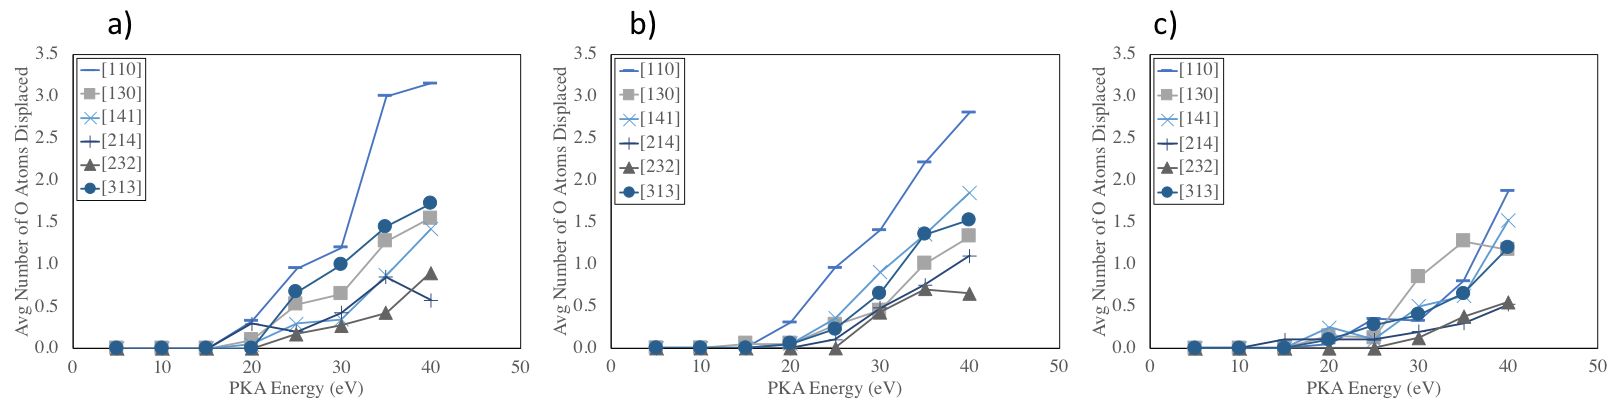
\includegraphics[width=1.0\textwidth]{dispO_O.png}
%DIFDELCMD <  %%%
\DIFdelendFL \DIFaddbeginFL 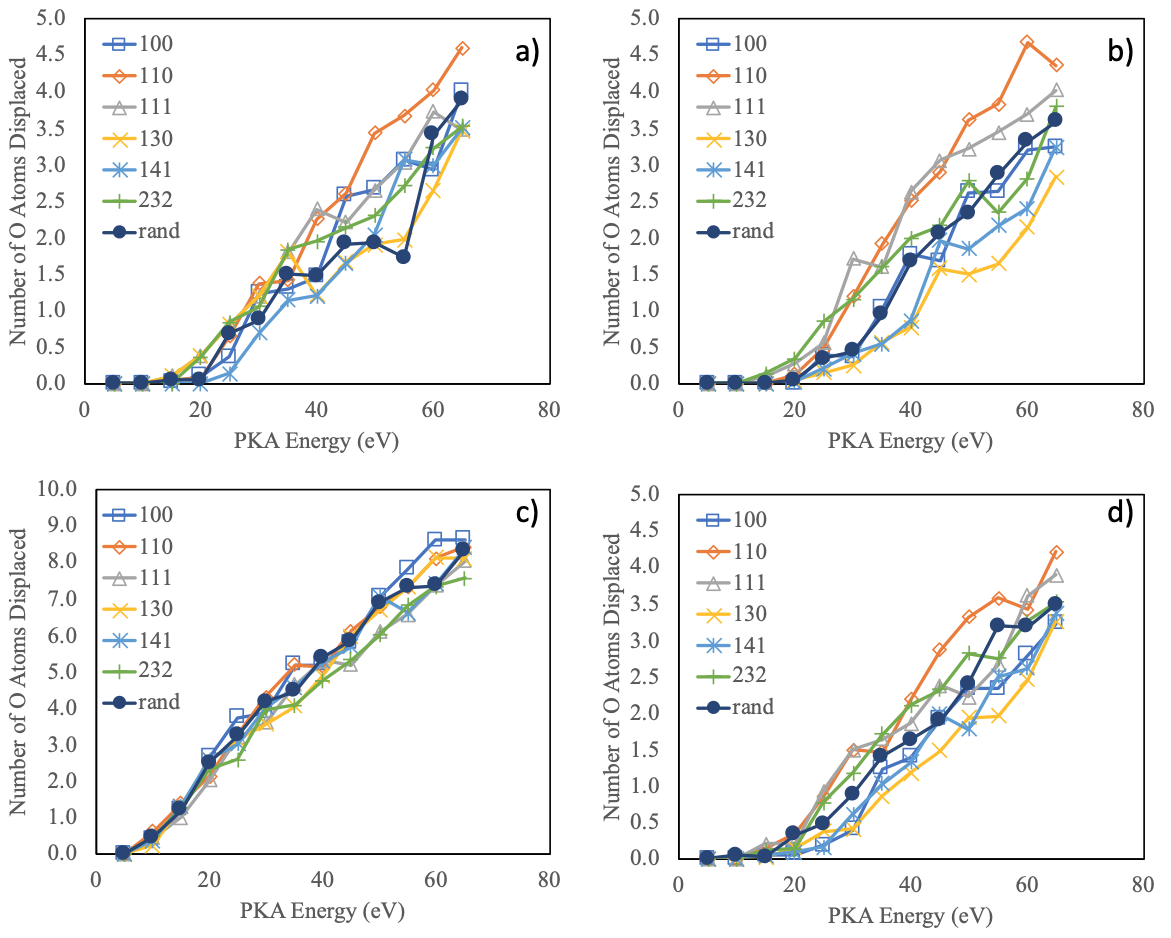
\includegraphics[width=1.0\textwidth]{disp_allO.png}
 \DIFaddendFL \caption{\DIFdelbeginFL \DIFdelFL{Average }\DIFdelendFL \DIFaddbeginFL \DIFaddFL{The }\DIFaddendFL number of \DIFdelbeginFL \DIFdelFL{oxygen }\DIFdelendFL \DIFaddbeginFL \DIFaddFL{O }\DIFaddendFL atoms \DIFaddbeginFL \DIFaddFL{permanently }\DIFaddendFL displaced \DIFaddbeginFL \DIFaddFL{in UO$_2$ }\DIFaddendFL by \DIFdelbeginFL \DIFdelFL{an }\DIFdelendFL O \DIFdelbeginFL \DIFdelFL{PKA as a function of PKA energy }\DIFdelendFL \DIFaddbeginFL \DIFaddFL{PKAs }\DIFaddendFL in \DIFdelbeginFL \DIFdelFL{$UO_2$ in }\DIFdelendFL the [\DIFaddbeginFL \DIFaddFL{100}]\DIFaddFL{, }[\DIFaddendFL 110], [\DIFdelbeginFL \DIFdelFL{130}\DIFdelendFL \DIFaddbeginFL \DIFaddFL{111}\DIFaddendFL ], [\DIFdelbeginFL \DIFdelFL{141}\DIFdelendFL \DIFaddbeginFL \DIFaddFL{130}\DIFaddendFL ], [\DIFdelbeginFL \DIFdelFL{214}\DIFdelendFL \DIFaddbeginFL \DIFaddFL{141}\DIFaddendFL ], [232] and \DIFdelbeginFL %DIFDELCMD < [%%%
\DIFdelFL{313}%DIFDELCMD < ] %%%
\DIFdelendFL \DIFaddbeginFL \DIFaddFL{random }\DIFaddendFL directions for the a) Basak, b) Yakub\DIFdelbeginFL \DIFdelFL{and }\DIFdelendFL \DIFaddbeginFL \DIFaddFL{, }\DIFaddendFL c) \DIFdelbeginFL \DIFdelFL{Yamada }\DIFdelendFL \DIFaddbeginFL \DIFaddFL{Morelon, and d) Cooper }\DIFaddendFL potentials. \DIFaddbeginFL \DIFaddFL{U atoms are not displaced by O PKAs in this energy range..}\DIFaddendFL }
 \DIFdelbeginFL %DIFDELCMD < \label{fig:dispoo}
%DIFDELCMD < %%%
\DIFdelendFL \DIFaddbeginFL \label{fig:dispallO}
\DIFaddendFL \end{figure*}

\FloatBarrier


\DIFdelbegin \subsubsection{\DIFdel{Displaced uranium atoms}}
%DIFAUXCMD
\addtocounter{subsubsection}{-1}%DIFAUXCMD
\DIFdel{\hspace{5mm}
}\DIFdelend \DIFaddbegin \subsection{\DIFadd{Probability of Frenkel pair formation}}
\DIFaddend 

\DIFdelbegin \DIFdel{The average number of uranium atoms permanently displaced per U PKA }\DIFdelend \DIFaddbegin \subsubsection{\DIFadd{Uranium PKA}}

\DIFadd{The probability of Frenkel pair formation }\DIFaddend as a function of PKA energy \DIFaddbegin \DIFadd{for U PKAs }\DIFaddend is shown in Fig. \DIFdelbegin \DIFdel{\ref{fig:dispuu}. Permanent displacement of atoms begins at a PKA energy of approximately 30 eV . Comparing to Fig. \ref{fig:dispou}, it requires an additional 10 eVof kinetic energy for a U atom to permanently displace another U atom, than for that U atom to displace an O atom. The }\DIFdelend \DIFaddbegin \DIFadd{\ref{fig:fpu}. Probabilities are observed to be zero up to approximately 20 eV for all interatomic potentials and directions. Above 20 eV, probabilities become non-zero and there is a clear directional dependence in the probability curves. Similar to the results in both section \ref{sect1} and section \ref{sect2}, the highest probability is observed for the }\DIFaddend [\DIFdelbegin \DIFdel{130}\DIFdelend \DIFaddbegin \DIFadd{100}\DIFaddend ] \DIFdelbegin \DIFdel{and }\DIFdelend \DIFaddbegin \DIFadd{direction. The value of E$_d$}\DIFaddend [\DIFdelbegin \DIFdel{141}\DIFdelend \DIFaddbegin \DIFadd{U}\DIFaddend ] \DIFdelbegin \DIFdel{directions show the highest number of displaced U atoms, which is in agreement with the results in Fig. \ref{fig:fpu} on Frenkel pair generation. The fewest U atoms are displaced for PKAs in the }\DIFdelend \DIFaddbegin \DIFadd{is determined to be 60 eV for each of the Basak, Yakub and Cooper potentials and is determined to be greater than 65 eV for the Morelon potential. The Morelon potential yields a maximum probability for the random directions of 0.42 for U PKAs with an energy of 65 eV.
}

\begin{figure*}[h]
 \centering
 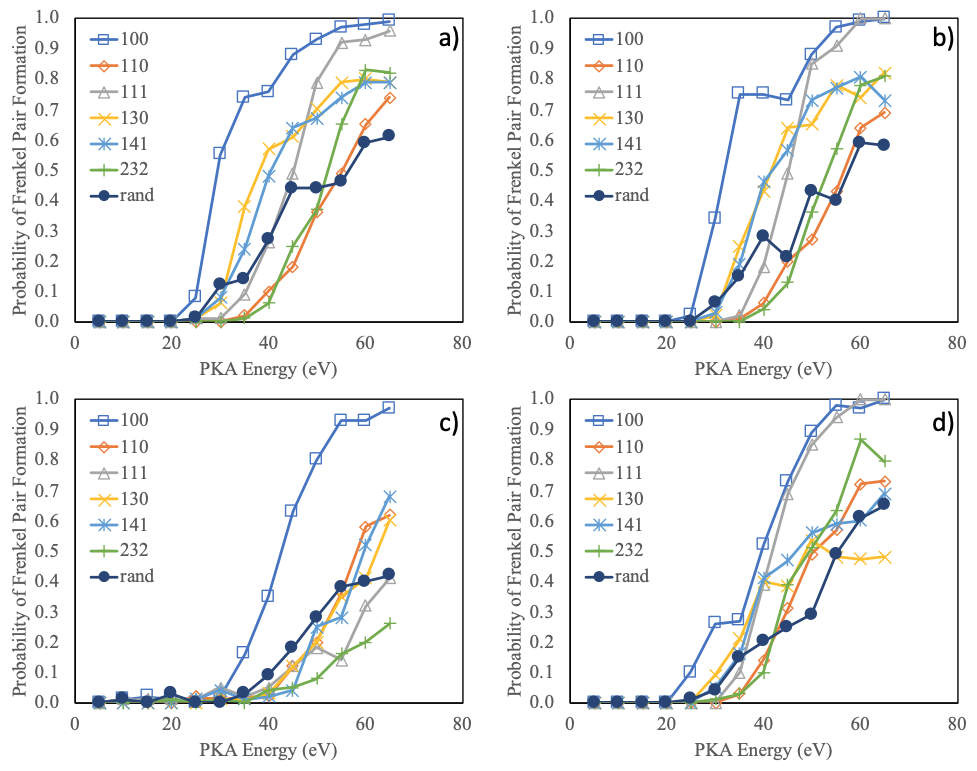
\includegraphics[width=1.0\textwidth]{FP_U.png}
 \caption{\DIFaddFL{Probability of Frenkel pair formation as a function of PKA energy in UO$_2$ for U PKAs in the }[\DIFaddFL{100}]\DIFaddFL{, }[\DIFaddFL{110}]\DIFaddFL{, }[\DIFaddFL{111}]\DIFaddFL{, }[\DIFaddFL{130}]\DIFaddFL{, }[\DIFaddFL{141}]\DIFaddFL{, }[\DIFaddFL{232}] \DIFaddFL{and random directions for the a) Basak, b) Yakub, c) Morelon, and d) Cooper potentials. }}
 \label{fig:fpu}
\end{figure*}

\FloatBarrier

\DIFadd{In addition to the probability of generating Frenkel pairs, the total number of Frenkel pairs is relevant to understanding a material's radiation response. Fig. \ref{fig:fpun} displays the total number of Frenkel pairs created. As expected, the total number of Frenkel pairs follows the same crystallographic trends as the probability to form Frenkel pairs from Fig. \ref{fig:fpu}. Utilizing the random set of directions to approximate average behavior and utilizing the secondary formalism of E$_d$ (when a PKA creates on average one Frenkel Pair), the value of E$_d$}\DIFaddend [\DIFdelbegin \DIFdel{214}\DIFdelend \DIFaddbegin \DIFadd{U}\DIFaddend ] \DIFdelbegin \DIFdel{direction, which is also in agreement with Fig. \ref{fig:fpu}. There is a general agreement on directional dependence and on the magnitude of displacements for all three potentials. For a U PKA of }\DIFdelend \DIFaddbegin \DIFadd{is }\DIFaddend 60 eV \DIFdelbegin \DIFdel{, the directionally-averaged number of displaced U atoms per }\DIFdelend \DIFaddbegin \DIFadd{for the Basak and Cooper potentials and greater than 65 eV for the Yakub the Morelon potentials. The maximum number of Frenkel pairs per PKA for a 65 eV }\DIFaddend U PKA is \DIFdelbegin \DIFdel{1.3, 1.1 and 1.2 for the Basak, Yakub and Yamada potentials, respectively.
Comparing to Fig. \ref{fig:dispou}, a U PKA of 60 eV will permanently displace approximately 4 times, 3 times or 8 times as many O atoms as U atoms for }\DIFdelend \DIFaddbegin \DIFadd{0.94 for the Yakub potential and 0.61 for the Morelon potential. This formalism for E$_d$}[\DIFadd{U}] \DIFadd{yields identical results for the Basak and Cooper potentials, but increases the magnitude of E$_d$ for the Yakub and Morelon potentials.
}

\begin{figure*}[h]
 \centering
 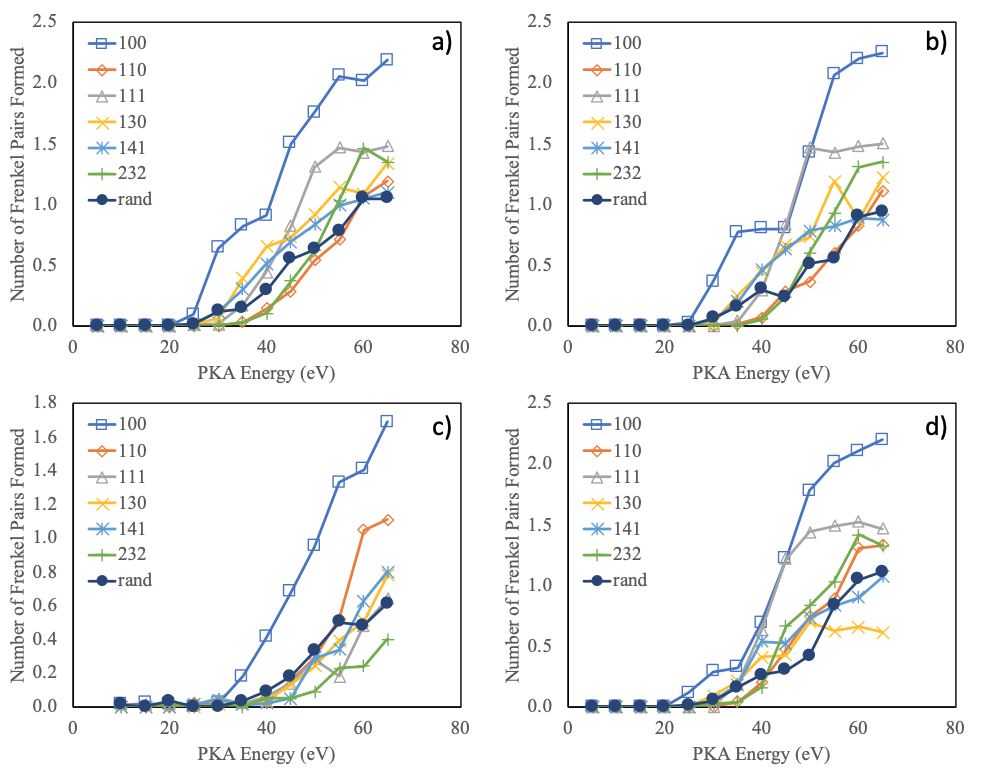
\includegraphics[width=1.0\textwidth]{FP_UN.png}
 \caption{\DIFaddFL{Total number of Frenkel pairs formed as a function of PKA energy in UO$_2$ for U PKAs in the }[\DIFaddFL{100}]\DIFaddFL{, }[\DIFaddFL{110}]\DIFaddFL{, }[\DIFaddFL{111}]\DIFaddFL{, }[\DIFaddFL{130}]\DIFaddFL{, }[\DIFaddFL{141}]\DIFaddFL{, }[\DIFaddFL{232}] \DIFaddFL{and random directions for the a) Basak, b) Yakub, c) Morelon, and d) Cooper potentials. }}
 \label{fig:fpun}
\end{figure*}

\FloatBarrier

\subsubsection{\DIFadd{Oxygen PKA}}

\DIFadd{The probability of Frenkel pair formation as a function of PKA energy for O PKAs is shown in Fig. \ref{fig:fpo}. Probabilities do not exceed 0.1 for any PKA energy with }\DIFaddend the Basak, Yakub and \DIFdelbegin \DIFdel{Yamada potentials, respectively. }%DIFDELCMD < 

%DIFDELCMD < %%%
\DIFdel{Permanently displaced U atoms due to an O PKA are not shown in this section, as the low energy }\DIFdelend \DIFaddbegin \DIFadd{Cooper potentials, and do not exceed 0.33 for the Morelon potential. Thus, it is never probable to form a Frenkel pair for O PKAs for energies below 65 eV. As such, E$_d$}[\DIFaddend O\DIFdelbegin \DIFdel{PKAs did not possess sufficient kinetic }\DIFdelend \DIFaddbegin ] \DIFadd{is undefinable, other than to note that it is greater than 65 eV. In this energy range, O PKAs are unable to transfer sufficient }\DIFaddend energy to displace \DIFdelbegin \DIFdel{a U atom from its original lattice site. }\DIFdelend \DIFaddbegin \DIFadd{uranium atoms, thus only a minimal number of O defects are formed. Albeit very minimal, probabilities do become non-zero at a PKA energies greater than 20 eV.
}\DIFaddend 

\begin{figure*}[h]
 \centering
 \DIFdelbeginFL %DIFDELCMD < 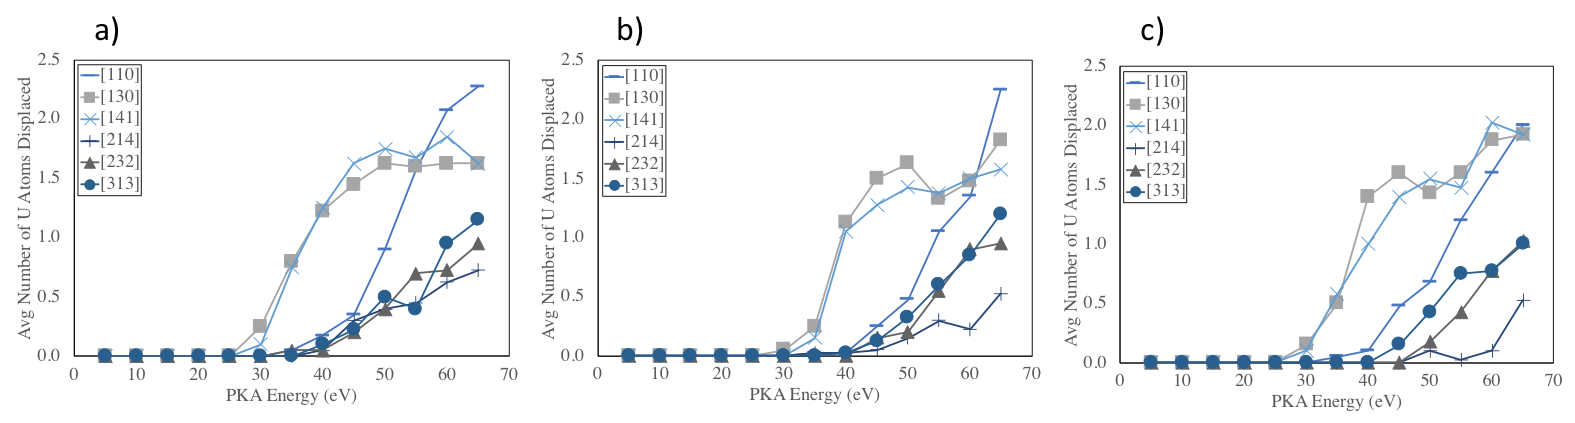
\includegraphics[width=1.0\textwidth]{dispU_U.png}
%DIFDELCMD <  %%%
\DIFdelendFL \DIFaddbeginFL 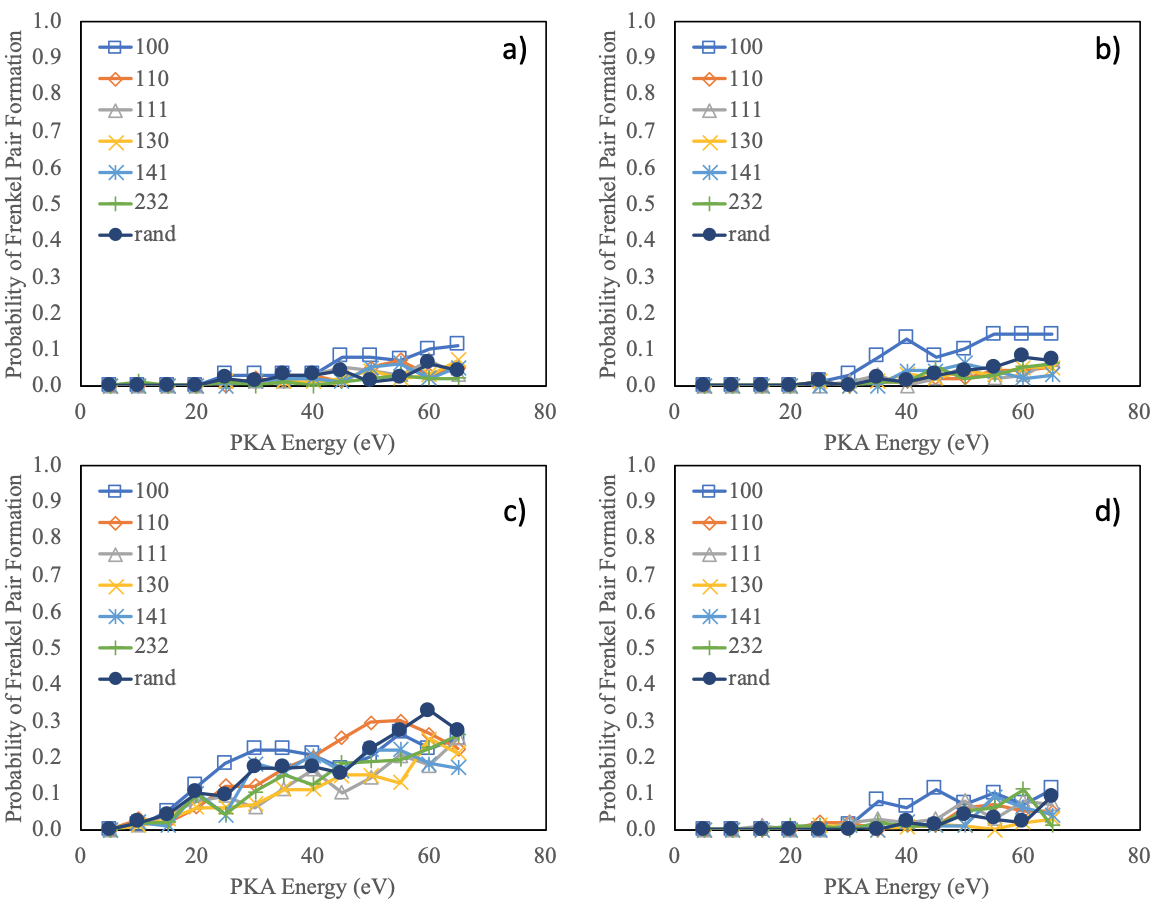
\includegraphics[width=1.0\textwidth]{FP_O.png}
 \DIFaddendFL \caption{\DIFdelbeginFL \DIFdelFL{Average number }\DIFdelendFL \DIFaddbeginFL \DIFaddFL{Probability }\DIFaddendFL of \DIFdelbeginFL \DIFdelFL{uranium atoms displaced by a U PKA }\DIFdelendFL \DIFaddbeginFL \DIFaddFL{Frenkel pair formation }\DIFaddendFL as a function of PKA energy in \DIFdelbeginFL \DIFdelFL{$UO_2$ }\DIFdelendFL \DIFaddbeginFL \DIFaddFL{UO$_2$ for O PKAs }\DIFaddendFL in the [\DIFaddbeginFL \DIFaddFL{100}]\DIFaddFL{, }[\DIFaddendFL 110], [\DIFdelbeginFL \DIFdelFL{130}\DIFdelendFL \DIFaddbeginFL \DIFaddFL{111}\DIFaddendFL ], [\DIFdelbeginFL \DIFdelFL{141}\DIFdelendFL \DIFaddbeginFL \DIFaddFL{130}\DIFaddendFL ], [\DIFdelbeginFL \DIFdelFL{214}\DIFdelendFL \DIFaddbeginFL \DIFaddFL{141}\DIFaddendFL ], [232] and \DIFdelbeginFL %DIFDELCMD < [%%%
\DIFdelFL{313}%DIFDELCMD < ] %%%
\DIFdelendFL \DIFaddbeginFL \DIFaddFL{random }\DIFaddendFL directions for the a) Basak, b) Yakub\DIFdelbeginFL \DIFdelFL{and }\DIFdelendFL \DIFaddbeginFL \DIFaddFL{, }\DIFaddendFL c) \DIFdelbeginFL \DIFdelFL{Yamada }\DIFdelendFL \DIFaddbeginFL \DIFaddFL{Morelon, and d) Cooper }\DIFaddendFL potentials. }
 \DIFdelbeginFL %DIFDELCMD < \label{fig:dispuu}
%DIFDELCMD < %%%
\DIFdelendFL \DIFaddbeginFL \label{fig:fpo}
\DIFaddendFL \end{figure*}

\FloatBarrier

\DIFdelbegin \subsection{\DIFdel{High energy oxygen PKA}}
%DIFAUXCMD
\addtocounter{subsection}{-1}%DIFAUXCMD
\DIFdel{\hspace{5mm}
}%DIFDELCMD < 

%DIFDELCMD < %%%
\DIFdelend In order to investigate the \DIFaddbegin \DIFadd{potential }\DIFaddend displacement of uranium atoms from an oxygen PKA, \DIFdelbegin \DIFdel{high energy (150-200 eV) oxygen PKAs }\DIFdelend \DIFaddbegin \DIFadd{higher energy O PKAs of up to 200 eV }\DIFaddend were utilized. \DIFdelbegin \DIFdel{As such, a full analysis of each formalism of the displacement energy was performed for the high energy O PKAs. }\DIFdelend Figure \ref{fig:fpoe} shows the probability of Frenkel pair formation as a function of O PKA energy \DIFdelbegin \DIFdel{. For each potential, there is a slight }\DIFdelend \DIFaddbegin \DIFadd{for the random direction and all four interatomic potentials. There is a }\DIFaddend positive trend of increasing defect probability with increasing PKA energy. \DIFdelbegin \DIFdel{Significantly, the Yamada potential predicts a dramatically higher Frenkel pair formation probability than either the Basak or Yakub potentials. At }\DIFdelend \DIFaddbegin \DIFadd{For the Basak, Yakub and Cooper potentials, the probability of generating a Frenkel pair from an O PKA of }\DIFaddend 200 eV \DIFdelbegin \DIFdel{, average probability of defect formation is 0.28, 0.26, and 0.72 for the Basak, Yakub and Yamada potentials, respectively. Thus, the Yamada potentialpredicts that a }\DIFdelend \DIFaddbegin \DIFadd{does not exceed 0.3. Thus, even for relatively high energy O PKAs, it is still unlikely to form a Frenkel pair. However, for the Morelon potential, the probability to create a Frenkel pair is significantly higher. A value for E$_d$}[\DIFadd{O}] \DIFadd{can be defined at 125 eV, where it becomes probable to create a Frenkel pair. It should be noted that these defects are almost entirely on the }\DIFaddend O \DIFdelbegin \DIFdel{PKA will produce approximately 2.5 times more Frenkel pairs than the same O PKA as predicted via the Basak or Yakub potentials. This substantial difference underlines the importance of understanding a given potential's behavior when conducting radiation damage simulations, given that similar potentials can produce dramatically different results. When comparing higher energy O PKAs }\DIFdelend \DIFaddbegin \DIFadd{sublattice. Thus, even though the kinetic energy of O atoms }\DIFaddend in Fig. \ref{fig:fpoe} \DIFdelbegin \DIFdel{to lower energy U PKAs }\DIFdelend \DIFaddbegin \DIFadd{is much higher than that of U atoms }\DIFaddend in Fig. \ref{fig:fpu}, it is \DIFdelbegin \DIFdel{observed that low energy U PKAs are still more likely to produce Frenkel pairs over these energy ranges (with the exception of results concerning the Yamada potential)}\DIFdelend \DIFaddbegin \DIFadd{much more probable to create Frenkel pairs from a U PKA}\DIFaddend .


\begin{figure*}[h]
 \centering
 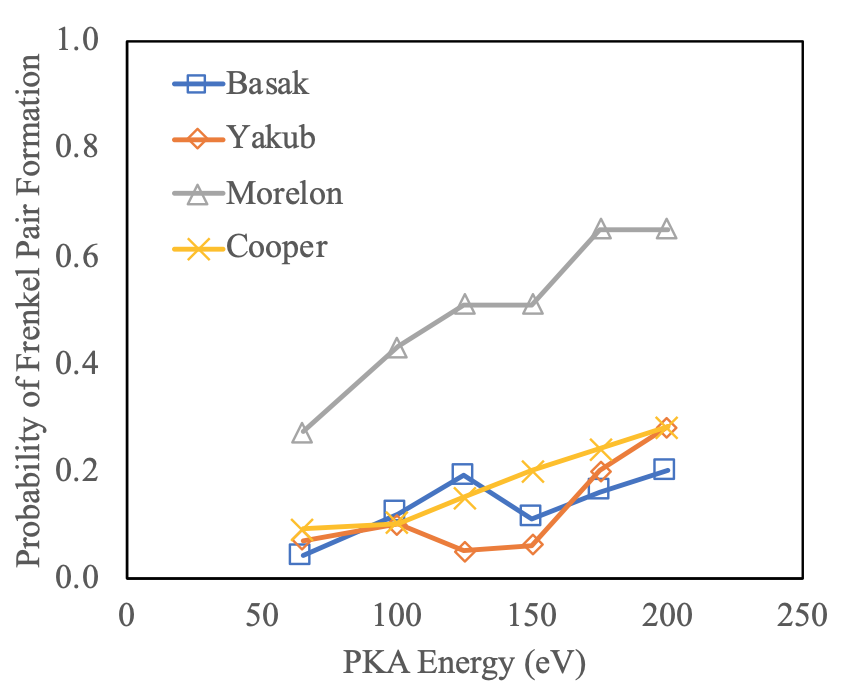
\includegraphics[width=1.0\textwidth]{FP_OE.png}
 \caption{Probability of Frenkel pair formation as a function of PKA energy \DIFdelbeginFL \DIFdelFL{in $UO_2$ due to }\DIFdelendFL \DIFaddbeginFL \DIFaddFL{for higher energy }\DIFaddendFL O PKAs in \DIFaddbeginFL \DIFaddFL{UO$_2$ in }\DIFaddendFL the \DIFdelbeginFL %DIFDELCMD < [%%%
\DIFdelFL{110}%DIFDELCMD < ]%%%
\DIFdelFL{, }%DIFDELCMD < [%%%
\DIFdelFL{130}%DIFDELCMD < ]%%%
\DIFdelFL{, }%DIFDELCMD < [%%%
\DIFdelFL{141}%DIFDELCMD < ]%%%
\DIFdelFL{, }%DIFDELCMD < [%%%
\DIFdelFL{214}%DIFDELCMD < ]%%%
\DIFdelFL{, }%DIFDELCMD < [%%%
\DIFdelFL{232}%DIFDELCMD < ] %%%
\DIFdelFL{and }%DIFDELCMD < [%%%
\DIFdelFL{313}%DIFDELCMD < ] %%%
\DIFdelFL{directions }\DIFdelendFL \DIFaddbeginFL \DIFaddFL{random direction }\DIFaddendFL for the a) Basak, b) Yakub\DIFdelbeginFL \DIFdelFL{and }\DIFdelendFL \DIFaddbeginFL \DIFaddFL{, }\DIFaddendFL c) \DIFdelbeginFL \DIFdelFL{Yamada }\DIFdelendFL \DIFaddbeginFL \DIFaddFL{Morelon, and d) Cooper }\DIFaddendFL potentials.}
 \label{fig:fpoe}
\end{figure*}

\DIFdelbegin \DIFdel{Table \ref{tab:dispU} shows the average number of displaced uranium atoms due to the high energy oxygen PKA. No uranium atoms were displaced in the  }%DIFDELCMD < [%%%
\DIFdel{110}%DIFDELCMD < ]%%%
\DIFdel{, }%DIFDELCMD < [%%%
\DIFdel{130}\DIFdelend \DIFaddbegin \FloatBarrier

\section{\DIFadd{Discussion}}

\DIFadd{A more clear comparison can be made by extracting the data for each set of random directions for each interatomic potential, PKA type, and E$_d$ definition. The consolidated results are shown in Table \ref{tab:Ed}, with the probability distributions shown for U PKAs in Fig. \ref{fig:pot_compU} and for O PKAs in Fig. \ref{fig:pot_compO}. In the table, the different definitions of E$_d$ are labeled E$_d^1$, E$_d^2$ and E$_d^3$, for the definitions of 1) the probability that a primary knock-on atom (PKA) leaves its original lattice site, 2) the probability that a PKA permanently displaces an atom from its original lattice site, and 3) the probability of forming a stable Frenkel pair. It is observed that results for the Basak, Yakub and Cooper potentials generally agree very well with one another, which the Morelon potential tends to exist as an outlier. The Morelon potential predicts lower probabilities for all three definitions of E$_d$}[\DIFadd{U}\DIFaddend ] \DIFdelbegin \DIFdel{, and }%DIFDELCMD < [%%%
\DIFdel{141}%DIFDELCMD < ] %%%
\DIFdel{PKA directions, thus they are excluded from the table. The O PKA energy range tested encompasses the minimum energy needed to transfer approximately 50 eV to the uranium atoms (with a direct collision). Due to this fact, the average number of uranium atoms displaced is very small, as at most a single uranium atom can be displaced in a given simulation. Additionally, there is not a monotonic increase of displacement probability . As U displacements from this energy range of O PKAs are rare events and thermal fluctuations are high in these systems (simulation temperature of 1500 K) , it is reasonable that there is significant statistical noise in the results . Although not statistically significant, the most likely PKA direction for U displacements is the }%DIFDELCMD < [%%%
\DIFdel{232}\DIFdelend \DIFaddbegin \DIFadd{and predicts higher probabilities for all three definitions  of E$_d$}[\DIFadd{O}\DIFaddend ]\DIFdelbegin \DIFdel{direction, and it is found that the Yakub potential is the most likely to show Udisplacements from these high energy OPKAs}\DIFdelend .

\DIFdelbegin %DIFDELCMD < \begin{table}[H]
%DIFDELCMD < 	%%%
\DIFdelendFL \DIFaddbeginFL \begin{figure*}[h]
 \centering
 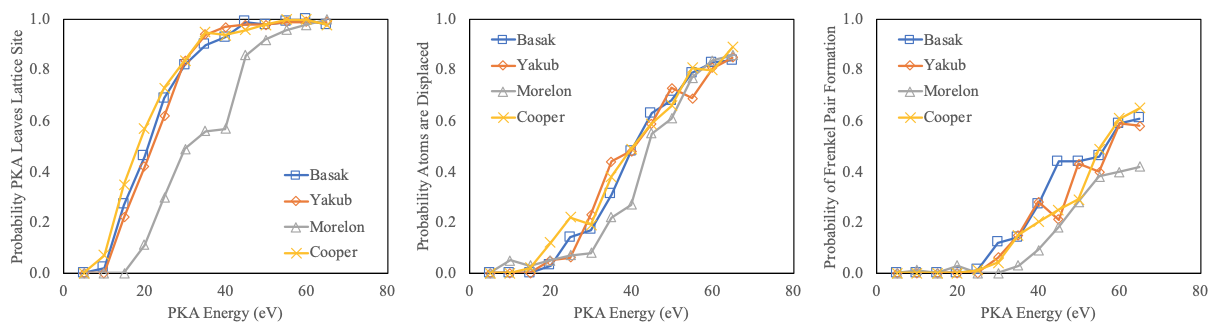
\includegraphics[width=1.0\textwidth]{pot_compU.png}
 \caption{\DIFaddFL{Probability PKA leaves lattice site, Probability atoms are displaced and Probability of Frenkel pair production as a function of U PKA energy for four interatomic potentials. }}
 \label{fig:pot_compU}
\end{figure*}

\begin{figure*}[h]
 \centering
 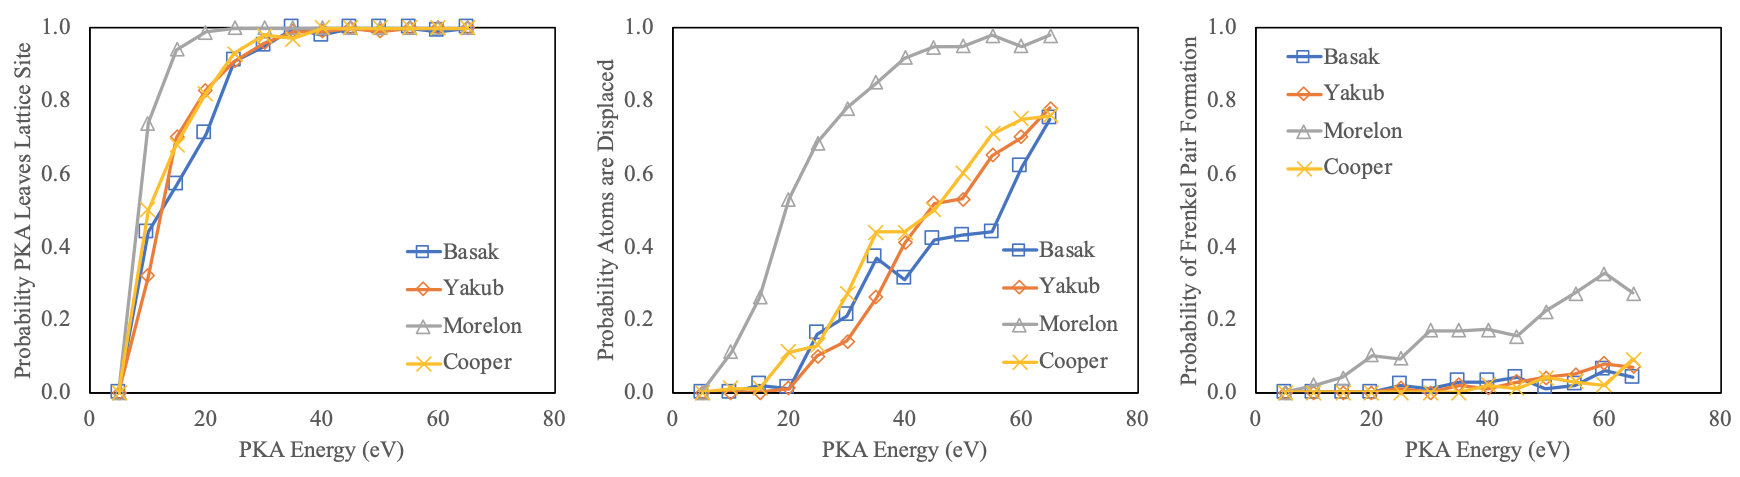
\includegraphics[width=1.0\textwidth]{pot_compO.png}
 \caption{ \DIFaddFL{Probability PKA leaves lattice site, Probability atoms are displaced and Probability of Frenkel pair production as a function of O PKA energy for four interatomic potentials. }}
 \label{fig:pot_compO}
\end{figure*}

\begin{table}[h]\label{tab:Ed}
	\DIFaddendFL \center
	\DIFdelbeginFL %DIFDELCMD < \begin{tabular}{|c||c|c|c|}
%DIFDELCMD < 		%%%
\DIFdelendFL \DIFaddbeginFL \caption{\DIFaddFL{The calculated displacement energies for four interatomic potentials, two PKA types and three different definitions of E$_d$.}}
	\begin{tabular}{|c|c|c|c|}
	
	 \DIFdelbeginFL \DIFdelFL{O PKA Energy (eV) }\DIFdelendFL & \DIFdelbeginFL %DIFDELCMD < [%%%
\DIFdelFL{214}%DIFDELCMD < ] %%%
\DIFdelendFL \DIFaddbeginFL \DIFaddFL{E$_d^1$ }\DIFaddendFL & \DIFdelbeginFL %DIFDELCMD < [%%%
\DIFdelFL{232}%DIFDELCMD < ] %%%
\DIFdelendFL \DIFaddbeginFL \DIFaddFL{E$_d^2$ }\DIFaddendFL & \DIFdelbeginFL %DIFDELCMD < [%%%
\DIFdelFL{313}%DIFDELCMD < ]%%%
\DIFdelendFL \DIFaddbeginFL \DIFaddFL{E$_d^3$ }\DIFaddendFL \\
	 \hline
	\DIFdelbeginFL %DIFDELCMD < \hline
%DIFDELCMD < 		 %%%
\DIFdelendFL \DIFaddbeginFL \DIFaddFL{Basak E$_d$}[\DIFaddFL{U}]	\DIFaddendFL & \DIFdelbeginFL \DIFdelFL{0 }\DIFdelendFL \DIFaddbeginFL \DIFaddFL{25 }\DIFaddendFL & \DIFdelbeginFL \DIFdelFL{0 }\DIFdelendFL \DIFaddbeginFL \DIFaddFL{45 }\DIFaddendFL & \DIFdelbeginFL \DIFdelFL{0}\DIFdelendFL \DIFaddbeginFL \DIFaddFL{60 }\DIFaddendFL \\
	\DIFdelbeginFL \DIFdelFL{150 }\DIFdelendFL \DIFaddbeginFL \DIFaddFL{Basak E$_d$}[\DIFaddFL{O}]	\DIFaddendFL & \DIFdelbeginFL \DIFdelFL{\textbf{0} }\DIFdelendFL \DIFaddbeginFL \DIFaddFL{15 }\DIFaddendFL & \DIFdelbeginFL \DIFdelFL{\textbf{0.075} }\DIFdelendFL \DIFaddbeginFL \DIFaddFL{60 }\DIFaddendFL & \DIFdelbeginFL \DIFdelFL{\textbf{0}}\DIFdelendFL \DIFaddbeginFL \DIFaddFL{$>$200 }\DIFaddendFL \\
	 \DIFdelbeginFL %DIFDELCMD < & %%%
\DIFdelFL{\textit{0} }%DIFDELCMD < & %%%
\DIFdelFL{\textit{0} }%DIFDELCMD < & %%%
\DIFdelFL{\textit{0}}%DIFDELCMD < \\
%DIFDELCMD < 		%%%

 	\DIFaddbeginFL \DIFaddFL{Yakub E$_d$}[\DIFaddFL{U}]	\DIFaddendFL & \DIFdelbeginFL \DIFdelFL{0 }\DIFdelendFL \DIFaddbeginFL \DIFaddFL{25 }\DIFaddendFL & \DIFdelbeginFL \DIFdelFL{0 }\DIFdelendFL \DIFaddbeginFL \DIFaddFL{45 }\DIFaddendFL & \DIFdelbeginFL \DIFdelFL{0}\DIFdelendFL \DIFaddbeginFL \DIFaddFL{60 }\DIFaddendFL \\
	\DIFdelbeginFL \DIFdelFL{160 }\DIFdelendFL \DIFaddbeginFL \DIFaddFL{Yakub E$_d$}[\DIFaddFL{O}]	\DIFaddendFL & \DIFdelbeginFL \DIFdelFL{\textbf{0} }\DIFdelendFL \DIFaddbeginFL \DIFaddFL{15 }\DIFaddendFL & \DIFdelbeginFL \DIFdelFL{\textbf{0} }\DIFdelendFL \DIFaddbeginFL \DIFaddFL{45 }\DIFaddendFL & \DIFdelbeginFL \DIFdelFL{\textbf{0}}\DIFdelendFL \DIFaddbeginFL \DIFaddFL{$>$200 }\DIFaddendFL \\
	 \DIFdelbeginFL %DIFDELCMD < & %%%
\DIFdelFL{\textit{0} }%DIFDELCMD < & %%%
\DIFdelFL{\textit{0} }%DIFDELCMD < & %%%
\DIFdelFL{\textit{0}}%DIFDELCMD < \\
%DIFDELCMD < 		%%%

	\DIFaddbeginFL \DIFaddFL{Morelon E$_d$}[\DIFaddFL{U}]	\DIFaddendFL & \DIFdelbeginFL \DIFdelFL{0 }\DIFdelendFL \DIFaddbeginFL \DIFaddFL{35 }\DIFaddendFL & \DIFdelbeginFL \DIFdelFL{0.05 }\DIFdelendFL \DIFaddbeginFL \DIFaddFL{45 }\DIFaddendFL & \DIFdelbeginFL \DIFdelFL{0}\DIFdelendFL \DIFaddbeginFL \DIFaddFL{$>$65 }\DIFaddendFL \\
	\DIFdelbeginFL \DIFdelFL{170 }\DIFdelendFL \DIFaddbeginFL \DIFaddFL{Morelon E$_d$}[\DIFaddFL{O}]	\DIFaddendFL & \DIFdelbeginFL \DIFdelFL{\textbf{0} }\DIFdelendFL \DIFaddbeginFL \DIFaddFL{10 }\DIFaddendFL & \DIFdelbeginFL \DIFdelFL{\textbf{0.025} }\DIFdelendFL \DIFaddbeginFL \DIFaddFL{20 }\DIFaddendFL & \DIFdelbeginFL \DIFdelFL{\textbf{0.1}}\DIFdelendFL \DIFaddbeginFL \DIFaddFL{125 }\DIFaddendFL \\
	 \DIFdelbeginFL %DIFDELCMD < & %%%
\DIFdelFL{\textit{0} }%DIFDELCMD < & %%%
\DIFdelFL{\textit{0} }%DIFDELCMD < & %%%
\DIFdelFL{\textit{0}}%DIFDELCMD < \\
%DIFDELCMD < 		%%%

	\DIFaddbeginFL \DIFaddFL{Cooper E$_d$}[\DIFaddFL{U}]	\DIFaddendFL & \DIFdelbeginFL \DIFdelFL{0 }\DIFdelendFL \DIFaddbeginFL \DIFaddFL{20 }\DIFaddendFL & \DIFdelbeginFL \DIFdelFL{0.05 }\DIFdelendFL \DIFaddbeginFL \DIFaddFL{45 }\DIFaddendFL & \DIFdelbeginFL \DIFdelFL{0}\DIFdelendFL \DIFaddbeginFL \DIFaddFL{60 }\DIFaddendFL \\
	\DIFdelbeginFL \DIFdelFL{180 }\DIFdelendFL \DIFaddbeginFL \DIFaddFL{Cooper E$_d$}[\DIFaddFL{O}]	\DIFaddendFL & \DIFdelbeginFL \DIFdelFL{\textbf{0} }\DIFdelendFL \DIFaddbeginFL \DIFaddFL{15 }\DIFaddendFL & \DIFdelbeginFL \DIFdelFL{\textbf{0} }\DIFdelendFL \DIFaddbeginFL \DIFaddFL{45 }\DIFaddendFL & \DIFdelbeginFL \DIFdelFL{\textbf{0.05}}%DIFDELCMD < \\
%DIFDELCMD < 		 & %%%
\DIFdelFL{\textit{0} }%DIFDELCMD < & %%%
\DIFdelFL{\textit{0} }%DIFDELCMD < & %%%
\DIFdelFL{\textit{0}}%DIFDELCMD < \\
%DIFDELCMD < 		\hline
%DIFDELCMD < 		 & %%%
\DIFdelFL{0.05 }%DIFDELCMD < & %%%
\DIFdelFL{0.175 }%DIFDELCMD < & %%%
\DIFdelFL{0}%DIFDELCMD < \\
%DIFDELCMD <        		%%%
\DIFdelFL{190 }%DIFDELCMD < & %%%
\DIFdelFL{\textbf{0} }%DIFDELCMD < & %%%
\DIFdelFL{\textbf{0.025} }%DIFDELCMD < & %%%
\DIFdelFL{\textbf{0.1}}%DIFDELCMD < \\
%DIFDELCMD < 		 & %%%
\DIFdelFL{\textit{0} }%DIFDELCMD < & %%%
\DIFdelFL{\textit{0} }%DIFDELCMD < & %%%
\DIFdelFL{\textit{0}}%DIFDELCMD < \\
%DIFDELCMD < 		\hline
%DIFDELCMD < 		 & %%%
\DIFdelFL{0 }%DIFDELCMD < & %%%
\DIFdelFL{0.15 }%DIFDELCMD < & %%%
\DIFdelFL{0}%DIFDELCMD < \\
%DIFDELCMD <        		%%%
\DIFdelendFL \DIFaddbeginFL \DIFaddFL{$>$}\DIFaddendFL 200 \DIFdelbeginFL %DIFDELCMD < & %%%
\DIFdelFL{\textbf{0.05} }%DIFDELCMD < & %%%
\DIFdelFL{\textbf{0.025} }%DIFDELCMD < & %%%
\DIFdelFL{\textbf{0}}\DIFdelendFL \\
	 \DIFdelbeginFL %DIFDELCMD < & %%%
\DIFdelFL{\textit{0} }%DIFDELCMD < & %%%
\DIFdelFL{\textit{0.05} }%DIFDELCMD < & %%%
\DIFdelFL{\textit{0}}%DIFDELCMD < \\
%DIFDELCMD < 		 %%%

	\end{tabular}
\DIFdelbeginFL %DIFDELCMD < \caption{%
{%DIFAUXCMD
\DIFdelFL{Average Number of Displaced Uranium Atoms by High Energy Oxygen PKA as a function of PKA energy and direction. The potentials are denoted by font styles: Basak, \textbf{Yakub}, and \textit{Yamada}.}}
	%DIFAUXCMD
%DIFDELCMD < \label{tab:dispU}
%DIFDELCMD < %%%
\DIFdelendFL \end{table}

\DIFdelbegin \DIFdel{Fig.\ref{fig:dispoe} shows the average number of displaced oxygen atoms due to the high energy oxygen PKAs. Similar to Fig. \ref{fig:fpoe} and Fig. \ref{fig:dispoo}, there is a positive trend of increasing number of displaced O atoms with increasing O PKA energy. Furthermore, the Yamada potential shows the highest number of displaced O atoms, while the Basak and Yakub show generally similar quantities of displaced Oatoms. For a 200 eVO PKA, the average number of displaced O atoms is 19}\DIFdelend \DIFaddbegin \DIFadd{The relative magnitude of the different definitions of E$_d$ make qualitative sense, in that it should be easiest to simply displace the PKA off of its lattice site and it should be most difficult to create a stable Frenkel pair. When comparing to the typically utilized values for E$_d$}[\DIFadd{U}] \DIFadd{of 40 eV and E$_d$}[\DIFadd{O}] \DIFadd{of 20 eV}\DIFaddend , \DIFdelbegin \DIFdel{15 and 25 for the Basak, Yakub and Yamada potentials, respectively.
}%DIFDELCMD < 

%DIFDELCMD < \begin{figure*}[h]
%DIFDELCMD <  \centering
%DIFDELCMD <  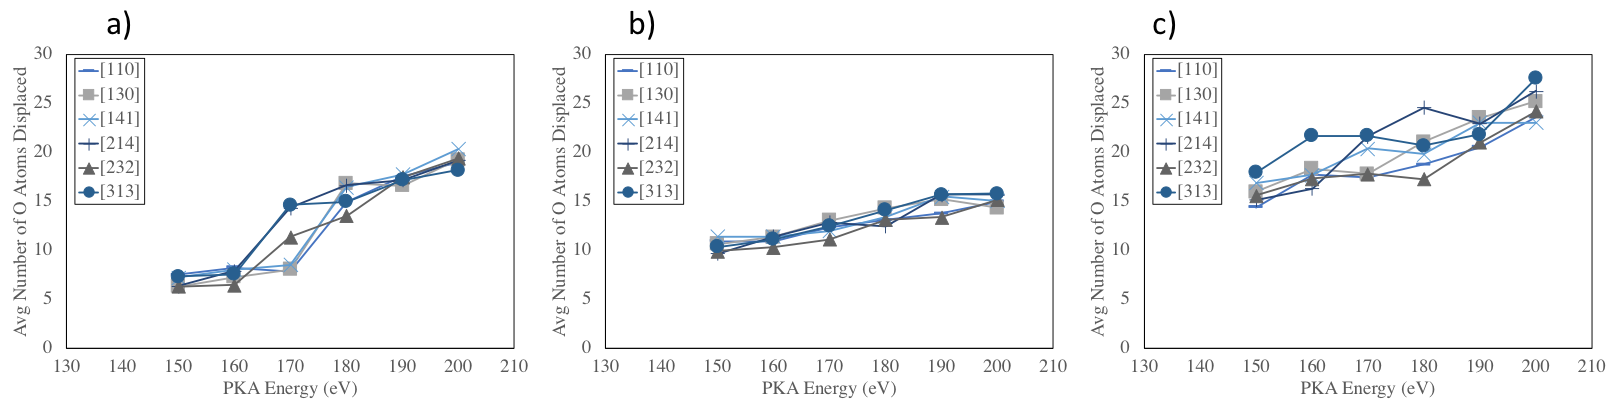
\includegraphics[width=1.0\textwidth]{dispO_OE.png}
%DIFDELCMD <  %%%
%DIFDELCMD < \caption{%
{%DIFAUXCMD
\DIFdelFL{Average number of oxygen atoms displaced by an O PKA as a function of PKA energy in $UO_2$ in the }%DIFDELCMD < [%%%
\DIFdelFL{110}%DIFDELCMD < ]%%%
\DIFdelFL{, }%DIFDELCMD < [%%%
\DIFdelFL{130}%DIFDELCMD < ]%%%
\DIFdelFL{, }%DIFDELCMD < [%%%
\DIFdelFL{141}%DIFDELCMD < ]%%%
\DIFdelFL{, }%DIFDELCMD < [%%%
\DIFdelFL{214}%DIFDELCMD < ]%%%
\DIFdelFL{, }%DIFDELCMD < [%%%
\DIFdelFL{232}%DIFDELCMD < ] %%%
\DIFdelFL{and }%DIFDELCMD < [%%%
\DIFdelFL{313}%DIFDELCMD < ] %%%
\DIFdelFL{directions for the a) Basak, b) Yakub and c) Yamada potentials.  }}
 %DIFAUXCMD
%DIFDELCMD < \label{fig:dispoe}
%DIFDELCMD < \end{figure*}
%DIFDELCMD < 

%DIFDELCMD < %%%
\section{\DIFdel{Discussion}}
%DIFAUXCMD
\addtocounter{section}{-1}%DIFAUXCMD
%DIFDELCMD < 

%DIFDELCMD < %%%
\DIFdel{This work has shown a consistency regarding the variation among the three interatomic potentials, in that they are in concordance when considering U PKAs, but the radiation damage properties vary significantly for the Yamada potential when considering O PKAs and the O sublattice. This is likely due to the oxygen sublattice properties defined by the Yamada potential. The Yamada potential exhibits properties of a more fluid oxygen sublattice, with significant distortion of O atoms off of the sublattice, in addition to rapid O interstitial diffusion. This was visually confirmed to be the case by use of Ovito \cite{ovito}. Because the Basak potential is considered an improvement of }\DIFdelend the \DIFdelbegin \DIFdel{Yamada potential \cite{basak}, and the Basak results generally agree with the Yakub potential , }\DIFdelend \DIFaddbegin \DIFadd{only set of results that provides a near match is for }\DIFaddend the \DIFdelbegin \DIFdel{Yamada potential is viewed as producing inaccurate oxygen sublattice behavior, and the authors would discourage the use of }\DIFdelend \DIFaddbegin \DIFadd{E$_d^2$ definition and }\DIFaddend the \DIFdelbegin \DIFdel{Yamada potential in high temperature radiation damagestudies}\DIFdelend \DIFaddbegin \DIFadd{Morelon potential, which as stated previously is the outlier in this dataset. However, the authors do believe the most relevant definition when comparing to these experimental results is likely E$_d^2$, which simply looks at permanent displacement of atoms, regardless or the production of defects. For this definition of E$_d$, this work points to values of E$_d$}[\DIFadd{O}] \DIFadd{and E$_d$}[\DIFadd{U}] \DIFadd{of approximately 45 eV. However, this number alone is not sufficient to understand the nature of the atoms that are displaced, as there are typically 5x more O atoms displaced than U atoms. Sublattice-specific displacements are important information, particularly because O atoms have been shown to be able to self-heal. It was also found that the minimum energy to displace a U atom is approximately 30 eV (from a U PKA) and the minimum energy to displace an O atom is approximately 10 eV (from a O PKA).
}

\DIFadd{The authors believe the most relevant definition of E$_d$ when trying to actually understand the results of radiation damage and potential deleterious effects on the material is E$_d^3$, which indicates the actual production of point defects. For this definition, E$_d$}[\DIFadd{U}] \DIFadd{is approximately 60 eV, and E$_d$}[\DIFadd{O}] \DIFadd{is higher than 200 eV. The authors believe this value, which allows for instantaneous ($<$5 ps) recombination of defects, is the appropriate value for utilization in the NRT equation for the calculation of radiation-induced damage}\DIFaddend .

\DIFaddbegin \FloatBarrier

\DIFaddend \section{Conclusion}
\hspace{5mm}

Molecular dynamics simulations of low energy PKAs have been performed to investigate the threshold displacement energy (\DIFdelbegin \DIFdel{$E_d$) in $UO_2$ }\DIFdelend \DIFaddbegin \DIFadd{E$_d$) in UO$_2$ }\DIFaddend at 1500 K. The Basak, Yakub\DIFdelbegin \DIFdel{and Yamada }\DIFdelend \DIFaddbegin \DIFadd{, Morelon and Cooper }\DIFaddend interatomic potentials were utilized. The \DIFdelbegin \DIFdel{$E_d$ was studied by looking at the probability of Frenkel pair production, }\DIFdelend \DIFaddbegin \DIFadd{E$_d$ was evaluated under three distinct definitions: 1) the probability that a primary knock-on atom (PKA) leaves its original lattice site, 2) }\DIFaddend the probability that \DIFdelbegin \DIFdel{the PKA leaves its lattice site and the number of permanently displaced atoms due to the PKA. Both uranium and oxygen }\DIFdelend \DIFaddbegin \DIFadd{a PKA permanently displaces an atom from its original lattice site, and 3) the probability of forming a stable Frenkel pair. Both U and O }\DIFaddend PKAs were utilized to \DIFdelbegin \DIFdel{investigate a broad scope of potential radiation damage in $UO_2$. Utilizing the definition of $E_d$ as the minimum energy required to form a stable Frenkel pair, it was found that the $E_d$ for U PKAs is 25-30 eV and the $E_d$ for O PKAs is 20-30 eV, depending on the interatomic potential utilized. These results are in agreement with experimental results for O atoms, but suggest a lower $E_d$ than the experimental value of 40 eV for U atoms. For utilization of the NRT equation, a median, directionally-averaged $E_d$ for U PKAs was calculated as approximately 55 eV. This quantity was not determined for O PKAs. It was found that the PKA}\DIFdelend \DIFaddbegin \DIFadd{develop species dependent values of E$_d$. It was found that the minimum }\DIFaddend energy \DIFdelbegin \DIFdel{required to permanently }\DIFdelend \DIFaddbegin \DIFadd{to displace a U atom is approximately 30 eV (from a U PKA) and the minimum energy to }\DIFaddend displace an O atom \DIFdelbegin \DIFdel{from its lattice site is approximately 20 eV , regardless of the PKAtype. Additionally, it requires 30 eV of kinetic energy for a U PKA to permanently displace a U atom from its lattice site. The minimum PKA energy observed for an O atom to displace a U atom is 150 eV. The results for the Basak and Yakub potentials were consistent for both U and O PKAsand showed only minimal variance across all simulated systems. The Yamada potential showed significant differences when compared to the Basak and Yakub potentials regarding O PKAs and properties of the O sublattice}\DIFdelend \DIFaddbegin \DIFadd{is approximately 10 eV (from a O PKA). For U PKAs, it becomes probable to displace an atom above an energy of approximately 45 eV and it becomes probable to create a defect at approximately 60 eV. For O PKAs, it becomes probable to displace an atom above an energy of approximately 45 eV and it does not become probable to create a defect at energies analyzed up to 200 eV}\DIFaddend . This work has provided the first insight into the high temperature nature of the \DIFdelbegin \DIFdel{threshold }\DIFdelend displacement energy in \DIFdelbegin \DIFdel{$UO_2$}\DIFdelend \DIFaddbegin \DIFadd{UO$_2$}\DIFaddend .



\DIFdelbegin %DIFDELCMD < \bibliographystyle{ieeetr}
%DIFDELCMD < %%%
\DIFdelend \bibliography{ref}

\end{document}
